%%%%%%%%%%%%%%%%%%%%%%%%%%%%%%%%%%%%%%%%%%%%%%%%%%%%%%%%%%%%%%%%%%%%%%%%%%
%%%%%%%%%%%%%%%%%%%%%%%%%%%%%%%%%%%%%%%%%%%%%%%%%%%%%%%%%%%%%%%%%%%%%%%%%%
\section{Appendix: Crosschecks Using Alternate ME-PS Matching And Factorization Scale Choices}
\label{sec:afmufsucrosschecks}
% ---- ---- ---- ---- ---- ---- ---- ---- ---- ---- ---- ---- ---- ---- ----

In order to confirm the rubustness and usefulness of the procedure used to construct the W+jets shape (Sec.~\ref{sec:wjetsShapeMatchingQ2}) we perform a series of cross-checks using alternative $f_\text{MatchingUp}$ and $f_\text{scaleUp}$ ($f_{MU}$ and $f_{SU}$) choices. Specifically, the fit is performed with:
\begin{itemize}
\item The Default W+jets sample (\textit{i.e.} $f_{MU}=0$, $f_{SU}=0$). The difference in the Diboson Yield vs the standard fit is $+26$ events, with the result shown in Fig.~\ref{fig:fsufmuXcheck_fSU0fMU0} and the full fit output of
{\tiny
\begin{verbatim}
 COVARIANCE MATRIX CALCULATED SUCCESSFULLY
 FCN=-419442 FROM HESSE     STATUS=OK             46 CALLS         211 TOTAL
                     EDM=4.42809e-07    STRATEGY= 1      ERROR MATRIX ACCURATE 
  EXT PARAMETER                                INTERNAL      INTERNAL  
  NO.   NAME      VALUE            ERROR       STEP SIZE       VALUE   
   1  nDiboson     1.76522e+03   3.71702e+02   3.99002e+00   1.76522e+03
   2  nQCD         1.20082e+02   3.17095e+02   3.71079e+00   1.20082e+02
   3  nSingleTop   6.52046e+02   3.26297e+01   2.89789e+00   6.52046e+02
   4  nTTbar       1.67593e+03   1.17108e+02   9.62779e+00   1.67593e+03
   5  nWjets       6.76408e+04   5.74577e+02   4.89037e+00   6.76408e+04
   6  nZjets       3.60548e+03   1.54811e+02   2.41198e+00   3.60548e+03
                               ERR DEF= 0.5
 EXTERNAL ERROR MATRIX.    NDIM=  25    NPAR=  6    ERR DEF=0.5
  1.382e+05 -2.384e+03 -1.402e+02 -2.441e+03 -1.277e+05 -2.485e+03 
 -2.384e+03  1.005e+05 -6.611e+00 -8.758e+01 -9.749e+04 -1.937e+02 
 -1.402e+02 -6.611e+00  1.065e+03 -4.304e+00 -9.126e+02  1.519e+00 
 -2.441e+03 -8.758e+01 -4.304e+00  1.371e+04 -1.118e+04  5.645e+01 
 -1.277e+05 -9.749e+04 -9.126e+02 -1.118e+04  3.301e+05 -2.122e+04 
 -2.485e+03 -1.937e+02  1.519e+00  5.645e+01 -2.122e+04  2.397e+04 
 PARAMETER  CORRELATION COEFFICIENTS  
       NO.  GLOBAL      1      2      3      4      5      6
        1  0.79899   1.000 -0.020 -0.012 -0.056 -0.598 -0.043
        2  0.75522  -0.020  1.000 -0.001 -0.002 -0.535 -0.004
        3  0.11819  -0.012 -0.001  1.000 -0.001 -0.049  0.000
        4  0.39314  -0.056 -0.002 -0.001  1.000 -0.166  0.003
        5  0.87893  -0.598 -0.535 -0.049 -0.166  1.000 -0.239
        6  0.49022  -0.043 -0.004  0.000  0.003 -0.239  1.000

  RooFitResult: minimized FCN value: -419442, estimated distance to minimum: 4.42809e-07
                covariance matrix quality: Full, accurate covariance matrix

    Constant Parameter    Value     
  --------------------  ------------
                   fMU    0.0000e+00
                   fSU    0.0000e+00

    Floating Parameter  InitialValue    FinalValue +/-  Error     GblCorr.
  --------------------  ------------  --------------------------  --------
              nDiboson    1.6969e+03    1.7652e+03 +/-  3.72e+02  <none>
                  nQCD    1.2256e+02    1.2008e+02 +/-  3.17e+02  <none>
            nSingleTop    6.5264e+02    6.5205e+02 +/-  3.26e+01  <none>
                nTTbar    1.6788e+03    1.6759e+03 +/-  1.17e+02  <none>
                nWjets    7.6129e+04    6.7641e+04 +/-  5.75e+02  <none>
                nZjets    3.6095e+03    3.6055e+03 +/-  1.55e+02  <none>

\end{verbatim}
}

\item The Scale Down sample (\textit{i.e.} $f_{MU}=0$, $f_{SU}=-1$). The difference in the Diboson Yield vs the standard fitis $+2139$ events, with the result shown in Fig.~\ref{fig:fsufmuXcheck_fSUm1fMU0} and the full fit output of
{\tiny
\begin{verbatim}
 COVARIANCE MATRIX CALCULATED SUCCESSFULLY
 FCN=-419332 FROM HESSE     STATUS=OK             40 CALLS         187 TOTAL
                     EDM=2.73019e-05    STRATEGY= 1      ERROR MATRIX ACCURATE 
  EXT PARAMETER                                INTERNAL      INTERNAL  
  NO.   NAME      VALUE            ERROR       STEP SIZE       VALUE   
   1  nDiboson     3.87457e+03   3.64117e+02   4.00537e+00   3.87457e+03
   2  nQCD         4.31214e+02   3.15714e+02   1.85041e+01   4.31214e+02
   3  nSingleTop   6.49209e+02   3.26296e+01   2.89778e+00   6.49209e+02
   4  nTTbar       1.57784e+03   1.17261e+02   9.64614e+00   1.57784e+03
   5  nWjets       6.51042e+04   5.59270e+02   4.88762e+00   6.51042e+04
   6  nZjets       3.81054e+03   1.54369e+02   1.20113e+01   3.81054e+03
                               ERR DEF= 0.5
 EXTERNAL ERROR MATRIX.    NDIM=  25    NPAR=  6    ERR DEF=0.5
  1.326e+05 -5.022e+03 -1.590e+02 -2.736e+03 -1.164e+05 -3.026e+03 
 -5.022e+03  9.968e+04  7.297e-01  7.829e+01 -9.416e+04 -4.581e+02 
 -1.590e+02  7.297e-01  1.065e+03 -2.086e+00 -9.014e+02  1.965e+00 
 -2.736e+03  7.829e+01 -2.086e+00  1.375e+04 -1.104e+04  8.015e+01 
 -1.164e+05 -9.416e+04 -9.014e+02 -1.104e+04  3.128e+05 -2.051e+04 
 -3.026e+03 -4.581e+02  1.965e+00  8.015e+01 -2.051e+04  2.383e+04 
 PARAMETER  CORRELATION COEFFICIENTS  
       NO.  GLOBAL      1      2      3      4      5      6
        1  0.78804   1.000 -0.044 -0.013 -0.064 -0.572 -0.054
        2  0.75467  -0.044  1.000  0.000  0.002 -0.533 -0.009
        3  0.11784  -0.013  0.000  1.000 -0.001 -0.049  0.000
        4  0.39164  -0.064  0.002 -0.001  1.000 -0.168  0.004
        5  0.87195  -0.572 -0.533 -0.049 -0.168  1.000 -0.238
        6  0.49228  -0.054 -0.009  0.000  0.004 -0.238  1.000

  RooFitResult: minimized FCN value: -419332, estimated distance to minimum: 2.73019e-05
                covariance matrix quality: Full, accurate covariance matrix

    Constant Parameter    Value     
  --------------------  ------------
                   fMU    0.0000e+00
                   fSU   -1.0000e+00

    Floating Parameter  InitialValue    FinalValue +/-  Error     GblCorr.
  --------------------  ------------  --------------------------  --------
              nDiboson    1.6969e+03    3.8746e+03 +/-  3.64e+02  <none>
                  nQCD    1.2256e+02    4.3121e+02 +/-  3.16e+02  <none>
            nSingleTop    6.5264e+02    6.4921e+02 +/-  3.26e+01  <none>
                nTTbar    1.6788e+03    1.5778e+03 +/-  1.17e+02  <none>
                nWjets    7.6129e+04    6.5104e+04 +/-  5.59e+02  <none>
                nZjets    3.6095e+03    3.8105e+03 +/-  1.54e+02  <none>

\end{verbatim}
}

\item The Scale Up sample (\textit{i.e.} $f_{MU}=0$, $f_{SU}=+1$). The difference in the Diboson Yield vs the standard fitis $-1053$ events, with the result shown in Fig.~\ref{fig:fsufmuXcheck_fSUp1fMU0} and the full fit output of
{\tiny
\begin{verbatim}
 COVARIANCE MATRIX CALCULATED SUCCESSFULLY
 FCN=-419367 FROM HESSE     STATUS=OK             50 CALLS         217 TOTAL
                     EDM=3.55243e-07    STRATEGY= 1      ERROR MATRIX ACCURATE 
  EXT PARAMETER                                INTERNAL      INTERNAL  
  NO.   NAME      VALUE            ERROR       STEP SIZE       VALUE   
   1  nDiboson     6.82883e+02   3.81608e+02   4.00860e+00   6.82883e+02
   2  nQCD         3.72757e+02   3.15472e+02   3.70255e+00   3.72757e+02
   3  nSingleTop   6.53154e+02   3.26277e+01   2.89760e+00   6.53154e+02
   4  nTTbar       1.67987e+03   1.17160e+02   1.92545e+00   1.67987e+03
   5  nWjets       6.83979e+04   5.83279e+02   4.89070e+00   6.83979e+04
   6  nZjets       3.65958e+03   1.54864e+02   2.40986e+00   3.65958e+03
                               ERR DEF= 0.5
 EXTERNAL ERROR MATRIX.    NDIM=  25    NPAR=  6    ERR DEF=0.5
  1.456e+05 -1.711e+03 -1.264e+02 -2.284e+03 -1.372e+05 -2.280e+03 
 -1.711e+03  9.952e+04 -1.032e+01 -1.279e+02 -9.697e+04 -3.697e+02 
 -1.264e+02 -1.032e+01  1.065e+03 -4.540e+00 -9.202e+02  9.472e-01 
 -2.284e+03 -1.279e+02 -4.540e+00  1.373e+04 -1.130e+04  4.112e+01 
 -1.372e+05 -9.697e+04 -9.202e+02 -1.130e+04  3.402e+05 -2.131e+04 
 -2.280e+03 -3.697e+02  9.472e-01  4.112e+01 -2.131e+04  2.398e+04 
 PARAMETER  CORRELATION COEFFICIENTS  
       NO.  GLOBAL      1      2      3      4      5      6
        1  0.80861   1.000 -0.014 -0.010 -0.051 -0.616 -0.039
        2  0.75388  -0.014  1.000 -0.001 -0.003 -0.527 -0.008
        3  0.11804  -0.010 -0.001  1.000 -0.001 -0.048  0.000
        4  0.39353  -0.051 -0.003 -0.001  1.000 -0.165  0.002
        5  0.88282  -0.616 -0.527 -0.048 -0.165  1.000 -0.236
        6  0.49140  -0.039 -0.008  0.000  0.002 -0.236  1.000

  RooFitResult: minimized FCN value: -419367, estimated distance to minimum: 3.55243e-07
                covariance matrix quality: Full, accurate covariance matrix

    Constant Parameter    Value     
  --------------------  ------------
                   fMU    0.0000e+00
                   fSU    1.0000e+00

    Floating Parameter  InitialValue    FinalValue +/-  Error     GblCorr.
  --------------------  ------------  --------------------------  --------
              nDiboson    1.6969e+03    6.8288e+02 +/-  3.82e+02  <none>
                  nQCD    1.2256e+02    3.7276e+02 +/-  3.15e+02  <none>
            nSingleTop    6.5264e+02    6.5315e+02 +/-  3.26e+01  <none>
                nTTbar    1.6788e+03    1.6799e+03 +/-  1.17e+02  <none>
                nWjets    7.6129e+04    6.8398e+04 +/-  5.83e+02  <none>
                nZjets    3.6095e+03    3.6596e+03 +/-  1.55e+02  <none>

\end{verbatim}
}


\item The Matching Down sample (\textit{i.e.} $f_{MU}=-1$, $f_{SU}=0$). The difference in the Diboson Yield vs the standard fitis $+865$ events, with the result shown in Fig.~\ref{fig:fsufmuXcheck_fSU0fMUm1} and the full fit output of
{\tiny
\begin{verbatim}
 COVARIANCE MATRIX CALCULATED SUCCESSFULLY
 FCN=-419341 FROM HESSE     STATUS=OK             40 CALLS         174 TOTAL
                     EDM=1.48026e-05    STRATEGY= 1      ERROR MATRIX ACCURATE 
  EXT PARAMETER                                INTERNAL      INTERNAL  
  NO.   NAME      VALUE            ERROR       STEP SIZE       VALUE   
   1  nDiboson     2.60131e+03   3.74192e+02   4.01399e+00   2.60131e+03
   2  nQCD         4.16151e+02   3.16071e+02   3.70053e+00   4.16151e+02
   3  nSingleTop   6.49785e+02   3.26308e+01   2.89775e+00   6.49785e+02
   4  nTTbar       1.59063e+03   1.17242e+02   9.64419e+00   1.59063e+03
   5  nWjets       6.64063e+04   5.72713e+02   4.88805e+00   6.64063e+04
   6  nZjets       3.78308e+03   1.54475e+02   1.20181e+01   3.78308e+03
                               ERR DEF= 0.5
 EXTERNAL ERROR MATRIX.    NDIM=  25    NPAR=  6    ERR DEF=0.5
  1.400e+05 -3.287e+03 -1.466e+02 -2.488e+03 -1.276e+05 -2.717e+03 
 -3.287e+03  9.990e+04 -2.140e+00  4.819e+01 -9.616e+04 -4.039e+02 
 -1.466e+02 -2.140e+00  1.065e+03 -2.508e+00 -9.110e+02  1.625e+00 
 -2.488e+03  4.819e+01 -2.508e+00  1.375e+04 -1.125e+04  7.352e+01 
 -1.276e+05 -9.616e+04 -9.110e+02 -1.125e+04  3.280e+05 -2.088e+04 
 -2.717e+03 -4.039e+02  1.625e+00  7.352e+01 -2.088e+04  2.386e+04 
 PARAMETER  CORRELATION COEFFICIENTS  
       NO.  GLOBAL      1      2      3      4      5      6
        1  0.79937   1.000 -0.028 -0.012 -0.057 -0.595 -0.047
        2  0.75508  -0.028  1.000 -0.000  0.001 -0.531 -0.008
        3  0.11794  -0.012 -0.000  1.000 -0.001 -0.049  0.000
        4  0.39161  -0.057  0.001 -0.001  1.000 -0.168  0.004
        5  0.87811  -0.595 -0.531 -0.049 -0.168  1.000 -0.236
        6  0.49229  -0.047 -0.008  0.000  0.004 -0.236  1.000

  RooFitResult: minimized FCN value: -419341, estimated distance to minimum: 1.48026e-05
                covariance matrix quality: Full, accurate covariance matrix

    Constant Parameter    Value     
  --------------------  ------------
                   fMU   -1.0000e+00
                   fSU    0.0000e+00

    Floating Parameter  InitialValue    FinalValue +/-  Error     GblCorr.
  --------------------  ------------  --------------------------  --------
              nDiboson    1.6969e+03    2.6013e+03 +/-  3.74e+02  <none>
                  nQCD    1.2256e+02    4.1615e+02 +/-  3.16e+02  <none>
            nSingleTop    6.5264e+02    6.4978e+02 +/-  3.26e+01  <none>
                nTTbar    1.6788e+03    1.5906e+03 +/-  1.17e+02  <none>
                nWjets    7.6129e+04    6.6406e+04 +/-  5.73e+02  <none>
                nZjets    3.6095e+03    3.7831e+03 +/-  1.54e+02  <none>

\end{verbatim}
}


\item The Matching Up sample (\textit{i.e.} $f_{MU}=+1$, $f_{SU}=0$). The difference in the Diboson Yield vs the standard fit is $-926$ events, with the result shown in Fig.~\ref{fig:fsufmuXcheck_fSU0fMUp1} and the full fit output of
{\tiny
\begin{verbatim}
 COVARIANCE MATRIX CALCULATED SUCCESSFULLY
 FCN=-419359 FROM HESSE     STATUS=OK             40 CALLS         189 TOTAL
                     EDM=7.79649e-05    STRATEGY= 1      ERROR MATRIX ACCURATE 
  EXT PARAMETER                                INTERNAL      INTERNAL  
  NO.   NAME      VALUE            ERROR       STEP SIZE       VALUE   
   1  nDiboson     8.09554e+02   3.79291e+02   4.00152e+00   8.09554e+02
   2  nQCD         3.34909e+02   3.16897e+02   3.70478e+00   3.34909e+02
   3  nSingleTop   6.51421e+02   3.26295e+01   2.89771e+00   6.51421e+02
   4  nTTbar       1.63606e+03   1.17185e+02   9.63594e+00   1.63606e+03
   5  nWjets       6.82674e+04   5.86978e+02   4.89196e+00   6.82674e+04
   6  nZjets       3.74038e+03   1.54532e+02   1.20281e+01   3.74038e+03
                               ERR DEF= 0.5
 EXTERNAL ERROR MATRIX.    NDIM=  25    NPAR=  6    ERR DEF=0.5
  1.439e+05 -2.951e+02 -1.183e+02 -2.195e+03 -1.373e+05 -2.088e+03 
 -2.951e+02  1.004e+05  7.034e-01  3.794e+01 -9.991e+04 -2.613e+02 
 -1.183e+02  7.034e-01  1.065e+03 -3.132e+00 -9.435e+02  2.079e+00 
 -2.195e+03  3.794e+01 -3.132e+00  1.373e+04 -1.156e+04  6.984e+01 
 -1.373e+05 -9.991e+04 -9.435e+02 -1.156e+04  3.445e+05 -2.163e+04 
 -2.088e+03 -2.613e+02  2.079e+00  6.984e+01 -2.163e+04  2.388e+04 
 PARAMETER  CORRELATION COEFFICIENTS  
       NO.  GLOBAL      1      2      3      4      5      6
        1  0.80708   1.000 -0.002 -0.010 -0.049 -0.617 -0.036
        2  0.75633  -0.002  1.000  0.000  0.001 -0.537 -0.005
        3  0.11814  -0.010  0.000  1.000 -0.001 -0.049  0.000
        4  0.39263  -0.049  0.001 -0.001  1.000 -0.168  0.004
        5  0.88427  -0.617 -0.537 -0.049 -0.168  1.000 -0.238
        6  0.49182  -0.036 -0.005  0.000  0.004 -0.238  1.000

  RooFitResult: minimized FCN value: -419359, estimated distance to minimum: 7.79649e-05
                covariance matrix quality: Full, accurate covariance matrix

    Constant Parameter    Value     
  --------------------  ------------
                   fMU    1.0000e+00
                   fSU    0.0000e+00

    Floating Parameter  InitialValue    FinalValue +/-  Error     GblCorr.
  --------------------  ------------  --------------------------  --------
              nDiboson    1.6969e+03    8.0955e+02 +/-  3.79e+02  <none>
                  nQCD    1.2256e+02    3.3491e+02 +/-  3.17e+02  <none>
            nSingleTop    6.5264e+02    6.5142e+02 +/-  3.26e+01  <none>
                nTTbar    1.6788e+03    1.6361e+03 +/-  1.17e+02  <none>
                nWjets    7.6129e+04    6.8267e+04 +/-  5.87e+02  <none>
                nZjets    3.6095e+03    3.7404e+03 +/-  1.55e+02  <none>

\end{verbatim}
}


\item Standard Fit parameters with $f_{SU}$ changed by $-1\sigma$. The difference in the Diboson Yield is $+119$ events, with the result shown in Fig.~\ref{fig:fsufmuXcheck_fSUm1sigmafMUDef} and the full fit output of
{\tiny
\begin{verbatim}
 COVARIANCE MATRIX CALCULATED SUCCESSFULLY
 FCN=-419443 FROM HESSE     STATUS=OK             40 CALLS         189 TOTAL
                     EDM=0.000159536    STRATEGY= 1      ERROR MATRIX ACCURATE 
  EXT PARAMETER                                INTERNAL      INTERNAL  
  NO.   NAME      VALUE            ERROR       STEP SIZE       VALUE   
   1  nDiboson     1.85540e+03   3.70770e+02   3.99120e+00   1.85540e+03
   2  nQCD         1.17997e+02   3.16657e+02   3.71104e+00   1.17997e+02
   3  nSingleTop   6.51466e+02   3.26290e+01   2.89794e+00   6.51466e+02
   4  nTTbar       1.66473e+03   1.17127e+02   9.63015e+00   1.66473e+03
   5  nWjets       6.75538e+04   5.72739e+02   4.89061e+00   6.75538e+04
   6  nZjets       3.61555e+03   1.54799e+02   1.20574e+01   3.61555e+03
                               ERR DEF= 0.5
 EXTERNAL ERROR MATRIX.    NDIM=  25    NPAR=  6    ERR DEF=0.5
  1.375e+05 -2.689e+03 -1.434e+02 -2.478e+03 -1.264e+05 -2.524e+03 
 -2.689e+03  1.003e+05 -5.225e+00 -6.854e+01 -9.692e+04 -1.551e+02 
 -1.434e+02 -5.225e+00  1.065e+03 -4.260e+00 -9.096e+02  1.995e+00 
 -2.478e+03 -6.854e+01 -4.260e+00  1.372e+04 -1.116e+04  6.135e+01 
 -1.264e+05 -9.692e+04 -9.096e+02 -1.116e+04  3.280e+05 -2.126e+04 
 -2.524e+03 -1.551e+02  1.995e+00  6.135e+01 -2.126e+04  2.396e+04 
 PARAMETER  CORRELATION COEFFICIENTS  
       NO.  GLOBAL      1      2      3      4      5      6
        1  0.79777   1.000 -0.023 -0.012 -0.057 -0.595 -0.044
        2  0.75465  -0.023  1.000 -0.001 -0.002 -0.534 -0.003
        3  0.11801  -0.012 -0.001  1.000 -0.001 -0.049  0.000
        4  0.39299  -0.057 -0.002 -0.001  1.000 -0.166  0.003
        5  0.87813  -0.595 -0.534 -0.049 -0.166  1.000 -0.240
        6  0.49075  -0.044 -0.003  0.000  0.003 -0.240  1.000

  RooFitResult: minimized FCN value: -419443, estimated distance to minimum: 0.000159536
                covariance matrix quality: Full, accurate covariance matrix

    Constant Parameter    Value     
  --------------------  ------------
                   fMU   -7.5000e-02
                   fSU   -2.5000e-02

    Floating Parameter  InitialValue    FinalValue +/-  Error     GblCorr.
  --------------------  ------------  --------------------------  --------
              nDiboson    1.6969e+03    1.8554e+03 +/-  3.71e+02  <none>
                  nQCD    1.2256e+02    1.1800e+02 +/-  3.17e+02  <none>
            nSingleTop    6.5264e+02    6.5147e+02 +/-  3.26e+01  <none>
                nTTbar    1.6788e+03    1.6647e+03 +/-  1.17e+02  <none>
                nWjets    7.6129e+04    6.7554e+04 +/-  5.73e+02  <none>
                nZjets    3.6095e+03    3.6156e+03 +/-  1.55e+02  <none>

\end{verbatim}
}


\item Standard Fit parameters with $f_{SU}$ changed by $+1\sigma$. The difference in the Diboson Yield is $-105$ events, with the result shown in Fig.~\ref{fig:fsufmuXcheck_fSUp1sigmafMUDef} and the full fit output of
{\tiny
\begin{verbatim}
 COVARIANCE MATRIX CALCULATED SUCCESSFULLY
 FCN=-419442 FROM HESSE     STATUS=OK             44 CALLS         211 TOTAL
                     EDM=3.83528e-07    STRATEGY= 1      ERROR MATRIX ACCURATE 
  EXT PARAMETER                                INTERNAL      INTERNAL  
  NO.   NAME      VALUE            ERROR       STEP SIZE       VALUE   
   1  nDiboson     1.63113e+03   3.73488e+02   3.99360e+00   1.63113e+03
   2  nQCD         1.23778e+02   3.17358e+02   3.71064e+00   1.23778e+02
   3  nSingleTop   6.51553e+02   3.26291e+01   2.89793e+00   6.51553e+02
   4  nTTbar       1.66447e+03   1.17162e+02   1.92600e+00   1.66447e+03
   5  nWjets       6.77743e+04   5.78430e+02   4.89051e+00   6.77743e+04
   6  nZjets       3.61414e+03   1.54934e+02   2.41157e+00   3.61414e+03
                               ERR DEF= 0.5
 EXTERNAL ERROR MATRIX.    NDIM=  25    NPAR=  6    ERR DEF=0.5
  1.395e+05 -1.897e+03 -1.344e+02 -2.364e+03 -1.301e+05 -2.329e+03 
 -1.897e+03  1.007e+05 -4.781e+00 -3.822e+01 -9.841e+04 -1.068e+02 
 -1.344e+02 -4.781e+00  1.065e+03 -3.845e+00 -9.207e+02  2.528e+00 
 -2.364e+03 -3.822e+01 -3.845e+00  1.373e+04 -1.133e+04  6.968e+01 
 -1.301e+05 -9.841e+04 -9.207e+02 -1.133e+04  3.346e+05 -2.160e+04 
 -2.329e+03 -1.068e+02  2.528e+00  6.968e+01 -2.160e+04  2.400e+04 
 PARAMETER  CORRELATION COEFFICIENTS  
       NO.  GLOBAL      1      2      3      4      5      6
        1  0.80095   1.000 -0.016 -0.011 -0.054 -0.602 -0.040
        2  0.75579  -0.016  1.000 -0.000 -0.001 -0.536 -0.002
        3  0.11802  -0.011 -0.000  1.000 -0.001 -0.049  0.001
        4  0.39315  -0.054 -0.001 -0.001  1.000 -0.167  0.004
        5  0.88053  -0.602 -0.536 -0.049 -0.167  1.000 -0.241
        6  0.49164  -0.040 -0.002  0.001  0.004 -0.241  1.000

  RooFitResult: minimized FCN value: -419442, estimated distance to minimum: 3.83528e-07
                covariance matrix quality: Full, accurate covariance matrix

    Constant Parameter    Value     
  --------------------  ------------
                   fMU   -7.5000e-02
                   fSU    1.3100e-01

    Floating Parameter  InitialValue    FinalValue +/-  Error     GblCorr.
  --------------------  ------------  --------------------------  --------
              nDiboson    1.6969e+03    1.6311e+03 +/-  3.73e+02  <none>
                  nQCD    1.2256e+02    1.2378e+02 +/-  3.17e+02  <none>
            nSingleTop    6.5264e+02    6.5155e+02 +/-  3.26e+01  <none>
                nTTbar    1.6788e+03    1.6645e+03 +/-  1.17e+02  <none>
                nWjets    7.6129e+04    6.7774e+04 +/-  5.78e+02  <none>
                nZjets    3.6095e+03    3.6141e+03 +/-  1.55e+02  <none>

\end{verbatim}
}


\item Standard Fit parameters with $f_{MU}$ changed by $-1\sigma$. The difference in the Diboson Yield is $+40$ events, with the result shown in Fig.~\ref{fig:fsufmuXcheck_fSUDeffMUm1sigma} and the full fit output of
{\tiny
\begin{verbatim}
 COVARIANCE MATRIX CALCULATED SUCCESSFULLY
 FCN=-419442 FROM HESSE     STATUS=OK             46 CALLS         211 TOTAL
                     EDM=4.15941e-07    STRATEGY= 1      ERROR MATRIX ACCURATE 
  EXT PARAMETER                                INTERNAL      INTERNAL  
  NO.   NAME      VALUE            ERROR       STEP SIZE       VALUE   
   1  nDiboson     1.77554e+03   3.71912e+02   3.99357e+00   1.77554e+03
   2  nQCD         1.20535e+02   3.15702e+02   3.71075e+00   1.20535e+02
   3  nSingleTop   6.51301e+02   3.26269e+01   2.89795e+00   6.51301e+02
   4  nTTbar       1.65848e+03   1.17135e+02   9.63113e+00   1.65848e+03
   5  nWjets       6.76333e+04   5.73141e+02   4.89038e+00   6.76333e+04
   6  nZjets       3.62073e+03   1.54638e+02   2.41123e+00   3.62073e+03
                               ERR DEF= 0.5
 EXTERNAL ERROR MATRIX.    NDIM=  25    NPAR=  6    ERR DEF=0.5
  1.383e+05 -2.508e+03 -1.384e+02 -2.427e+03 -1.276e+05 -2.561e+03 
 -2.508e+03  9.967e+04 -4.497e+00 -6.812e+01 -9.638e+04 -1.662e+02 
 -1.384e+02 -4.497e+00  1.065e+03 -4.345e+00 -9.129e+02  2.098e+00 
 -2.427e+03 -6.812e+01 -4.345e+00  1.372e+04 -1.120e+04  5.646e+01 
 -1.276e+05 -9.638e+04 -9.129e+02 -1.120e+04  3.285e+05 -2.111e+04 
 -2.561e+03 -1.662e+02  2.098e+00  5.646e+01 -2.111e+04  2.391e+04 
 PARAMETER  CORRELATION COEFFICIENTS  
       NO.  GLOBAL      1      2      3      4      5      6
        1  0.79914   1.000 -0.021 -0.011 -0.056 -0.599 -0.045
        2  0.75347  -0.021  1.000 -0.000 -0.002 -0.533 -0.003
        3  0.11779  -0.011 -0.000  1.000 -0.001 -0.049  0.000
        4  0.39289  -0.056 -0.002 -0.001  1.000 -0.167  0.003
        5  0.87843  -0.599 -0.533 -0.049 -0.167  1.000 -0.238
        6  0.48975  -0.045 -0.003  0.000  0.003 -0.238  1.000

  RooFitResult: minimized FCN value: -419442, estimated distance to minimum: 4.15941e-07
                covariance matrix quality: Full, accurate covariance matrix

    Constant Parameter    Value     
  --------------------  ------------
                   fMU   -1.4000e-01
                   fSU    5.3000e-02

    Floating Parameter  InitialValue    FinalValue +/-  Error     GblCorr.
  --------------------  ------------  --------------------------  --------
              nDiboson    1.6969e+03    1.7755e+03 +/-  3.72e+02  <none>
                  nQCD    1.2256e+02    1.2053e+02 +/-  3.16e+02  <none>
            nSingleTop    6.5264e+02    6.5130e+02 +/-  3.26e+01  <none>
                nTTbar    1.6788e+03    1.6585e+03 +/-  1.17e+02  <none>
                nWjets    7.6129e+04    6.7633e+04 +/-  5.73e+02  <none>
                nZjets    3.6095e+03    3.6207e+03 +/-  1.55e+02  <none>

\end{verbatim}
}


\item Standard Fit parameters with $f_{MU}$ changed by $+1\sigma$. The difference in the Diboson Yield is $-38$ events, with the result shown in Fig.~\ref{fig:fsufmuXcheck_fSUDeffMUp1sigma} and the full fit output of
{\tiny
\begin{verbatim}
 COVARIANCE MATRIX CALCULATED SUCCESSFULLY
 FCN=-419442 FROM HESSE     STATUS=OK             46 CALLS         213 TOTAL
                     EDM=4.17954e-07    STRATEGY= 1      ERROR MATRIX ACCURATE 
  EXT PARAMETER                                INTERNAL      INTERNAL  
  NO.   NAME      VALUE            ERROR       STEP SIZE       VALUE   
   1  nDiboson     1.69756e+03   3.71418e+02   3.99107e+00   1.69756e+03
   2  nQCD         1.20757e+02   3.16627e+02   3.71075e+00   1.20757e+02
   3  nSingleTop   6.51939e+02   3.26287e+01   2.89790e+00   6.51939e+02
   4  nTTbar       1.67357e+03   1.17206e+02   1.92565e+00   1.67357e+03
   5  nWjets       6.77091e+04   5.74880e+02   4.89044e+00   6.77091e+04
   6  nZjets       3.60658e+03   1.54900e+02   2.41193e+00   3.60658e+03
                               ERR DEF= 0.5
 EXTERNAL ERROR MATRIX.    NDIM=  25    NPAR=  6    ERR DEF=0.5
  1.380e+05 -2.072e+03 -1.338e+02 -2.487e+03 -1.279e+05 -2.473e+03 
 -2.072e+03  1.003e+05 -7.814e+00 -1.038e+02 -9.754e+04 -1.226e+02 
 -1.338e+02 -7.814e+00  1.065e+03 -5.135e+00 -9.162e+02  1.752e+00 
 -2.487e+03 -1.038e+02 -5.135e+00  1.374e+04 -1.112e+04  4.292e+01 
 -1.279e+05 -9.754e+04 -9.162e+02 -1.112e+04  3.305e+05 -2.135e+04 
 -2.473e+03 -1.226e+02  1.752e+00  4.292e+01 -2.135e+04  2.399e+04 
 PARAMETER  CORRELATION COEFFICIENTS  
       NO.  GLOBAL      1      2      3      4      5      6
        1  0.79885   1.000 -0.018 -0.011 -0.057 -0.599 -0.043
        2  0.75467  -0.018  1.000 -0.001 -0.003 -0.536 -0.003
        3  0.11804  -0.011 -0.001  1.000 -0.001 -0.049  0.000
        4  0.39338  -0.057 -0.003 -0.001  1.000 -0.165  0.002
        5  0.87904  -0.599 -0.536 -0.049 -0.165  1.000 -0.240
        6  0.49089  -0.043 -0.003  0.000  0.002 -0.240  1.000

  RooFitResult: minimized FCN value: -419442, estimated distance to minimum: 4.17954e-07
                covariance matrix quality: Full, accurate covariance matrix

    Constant Parameter    Value     
  --------------------  ------------
                   fMU   -1.0100e-02
                   fSU    5.3000e-02

    Floating Parameter  InitialValue    FinalValue +/-  Error     GblCorr.
  --------------------  ------------  --------------------------  --------
              nDiboson    1.6969e+03    1.6976e+03 +/-  3.71e+02  <none>
                  nQCD    1.2256e+02    1.2076e+02 +/-  3.17e+02  <none>
            nSingleTop    6.5264e+02    6.5194e+02 +/-  3.26e+01  <none>
                nTTbar    1.6788e+03    1.6736e+03 +/-  1.17e+02  <none>
                nWjets    7.6129e+04    6.7709e+04 +/-  5.75e+02  <none>
                nZjets    3.6095e+03    3.6066e+03 +/-  1.55e+02  <none>

\end{verbatim}
}


\item The standard muon fit parameters applied to the electron sample. The difference between the resultant and standard Diboson Yield in the electron channel is $-117$ events, with the result shown in Fig.~\ref{fig:fsufmuXcheck_fMUfSUMuonDefault} and the full fit output of
{\tiny
\begin{verbatim}
 COVARIANCE MATRIX CALCULATED SUCCESSFULLY
 FCN=-192969 FROM HESSE     STATUS=OK             40 CALLS         189 TOTAL
                     EDM=9.6052e-05    STRATEGY= 1      ERROR MATRIX ACCURATE 
  EXT PARAMETER                                INTERNAL      INTERNAL  
  NO.   NAME      VALUE            ERROR       STEP SIZE       VALUE   
   1  nDiboson     6.10378e+02   2.71262e+02   1.95137e+00   6.10378e+02
   2  nQCD         3.16333e+03   7.78822e+02   2.34592e+00   3.16333e+03
   3  nSingleTop   3.31940e+02   1.65915e+01   1.00307e+00   3.31940e+02
   4  nTTbar       9.54955e+02   6.72181e+01   3.85841e+00   9.54955e+02
   5  nWjets       3.28621e+04   7.87905e+02   2.39527e+00   3.28621e+04
   6  nZjets       1.48499e+03   6.38833e+01   3.68909e+00   1.48499e+03
                               ERR DEF= 0.5
 EXTERNAL ERROR MATRIX.    NDIM=  25    NPAR=  6    ERR DEF=0.5
  7.358e+04 -4.427e+04 -4.200e+01 -1.115e+03 -2.664e+04 -2.108e+02 
 -4.427e+04  6.066e+05  5.126e+01  1.371e+03 -5.556e+05 -1.710e+03 
 -4.200e+01  5.126e+01  2.753e+02 -1.018e+00 -2.810e+02  7.307e-02 
 -1.115e+03  1.371e+03 -1.018e+00  4.518e+03 -4.734e+03  3.090e+00 
 -2.664e+04 -5.556e+05 -2.810e+02 -4.734e+03  6.208e+05 -2.140e+03 
 -2.108e+02 -1.710e+03  7.307e-02  3.090e+00 -2.140e+03  4.081e+03 
 PARAMETER  CORRELATION COEFFICIENTS  
       NO.  GLOBAL      1      2      3      4      5      6
        1  0.80501   1.000 -0.210 -0.009 -0.061 -0.125 -0.012
        2  0.96867  -0.210  1.000  0.004  0.026 -0.905 -0.034
        3  0.08333  -0.009  0.004  1.000 -0.001 -0.021  0.000
        4  0.32358  -0.061  0.026 -0.001  1.000 -0.089  0.001
        5  0.96806  -0.125 -0.905 -0.021 -0.089  1.000 -0.043
        6  0.30645  -0.012 -0.034  0.000  0.001 -0.043  1.000

  RooFitResult: minimized FCN value: -192969, estimated distance to minimum: 9.6052e-05
                covariance matrix quality: Full, accurate covariance matrix

    Constant Parameter    Value     
  --------------------  ------------
                   fMU   -7.5000e-02
                   fSU    5.3300e-02

    Floating Parameter  InitialValue    FinalValue +/-  Error     GblCorr.
  --------------------  ------------  --------------------------  --------
              nDiboson    8.6705e+02    6.1038e+02 +/-  2.71e+02  <none>
                  nQCD    2.6099e+03    3.1633e+03 +/-  7.79e+02  <none>
            nSingleTop    3.3186e+02    3.3194e+02 +/-  1.66e+01  <none>
                nTTbar    9.6254e+02    9.5495e+02 +/-  6.72e+01  <none>
                nWjets    3.7137e+04    3.2862e+04 +/-  7.88e+02  <none>
                nZjets    1.4865e+03    1.4850e+03 +/-  6.39e+01  <none>

\end{verbatim}
}

\end{itemize}

As expected, using purely alternate samples yields large discrepancies in the diboson event counts and fit results; while changing the sample fractions by their uncertainties or fitting the electron channel using muon parameters produces output within the standard fit uncertainty.


%%%%%%%%%%%%%%%%%%%%
%%%%%%%%%%%%%%%%%%%%
\begin{figure}[h!]
  {\centering
    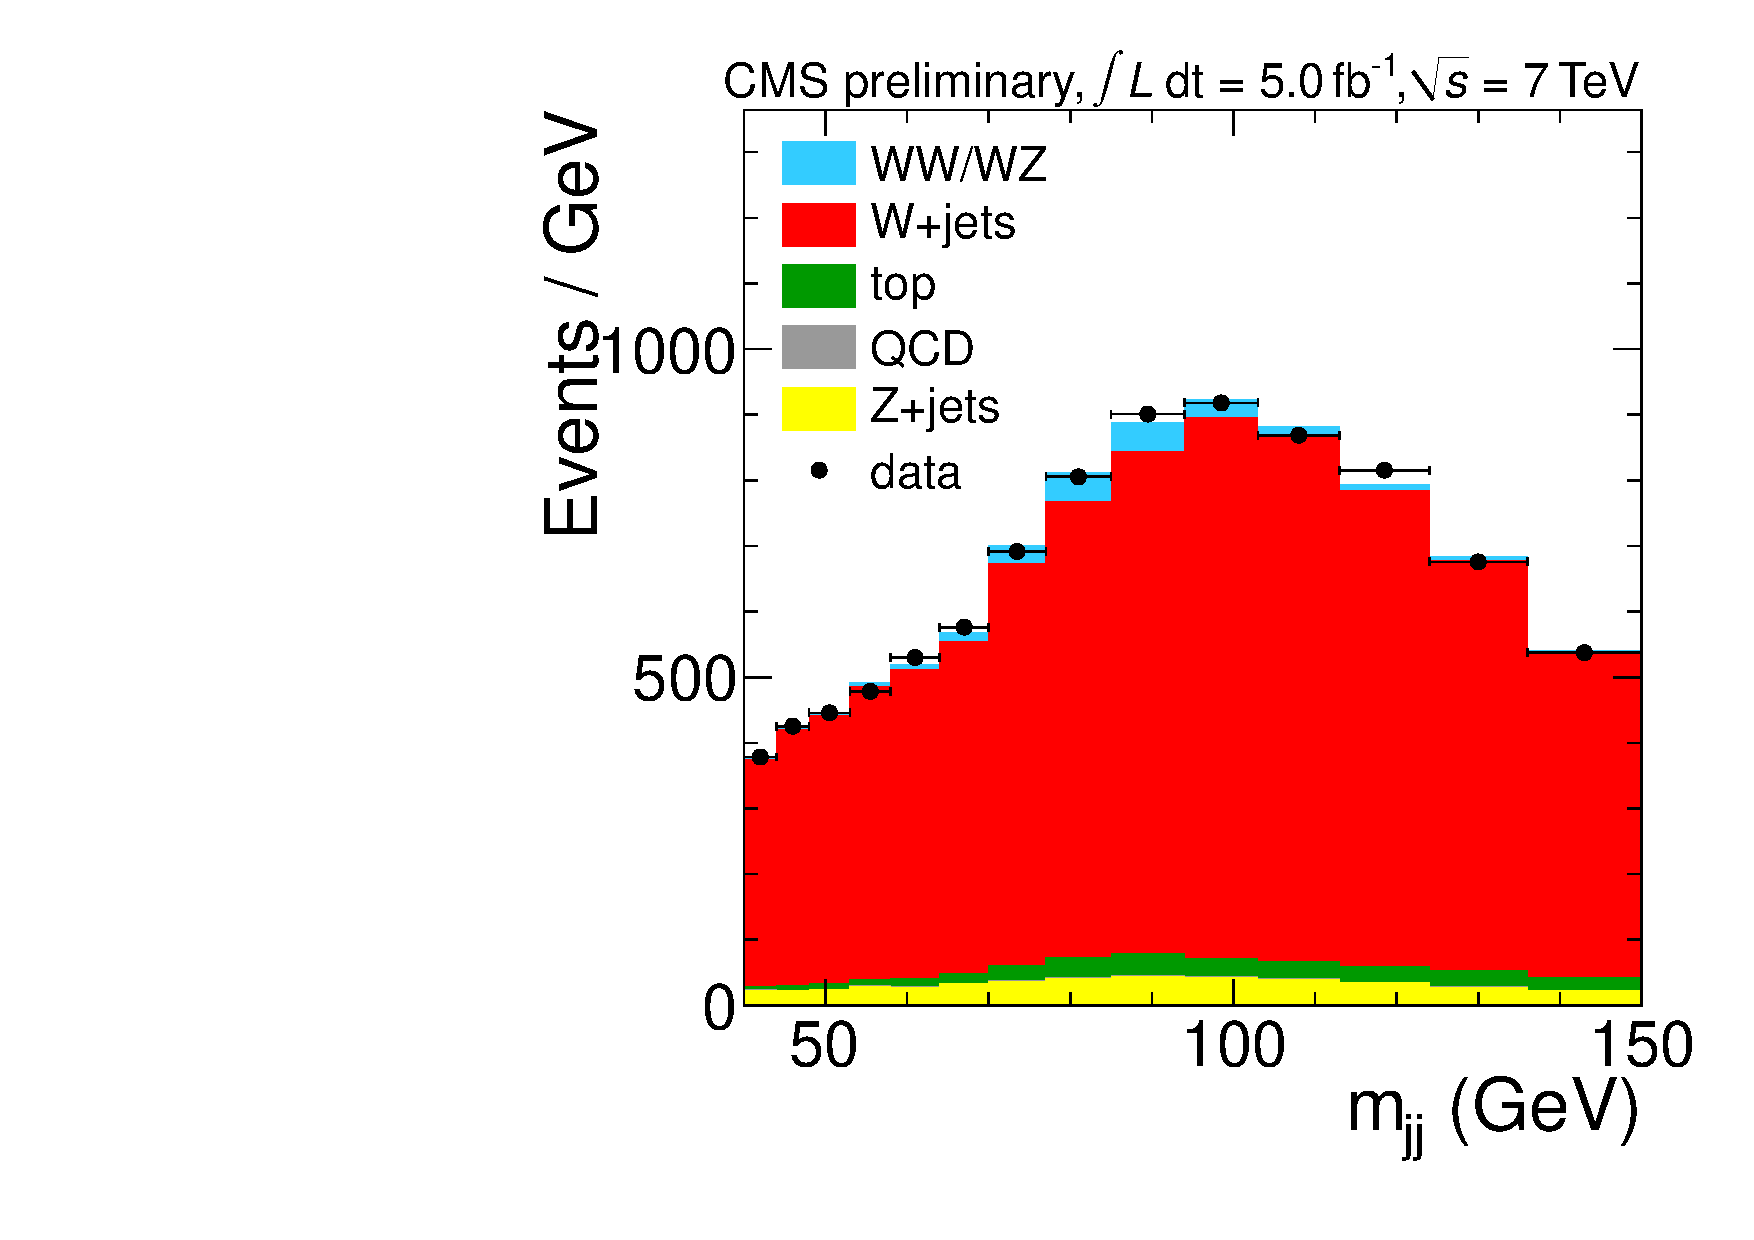
\includegraphics[width=0.49\textwidth]{figs/ScaleAndMatchingCrossChecks/mu2JNoBTag_fSU0fMU0/Wjj_Diboson_Muon_2jets_Stacked.pdf}
    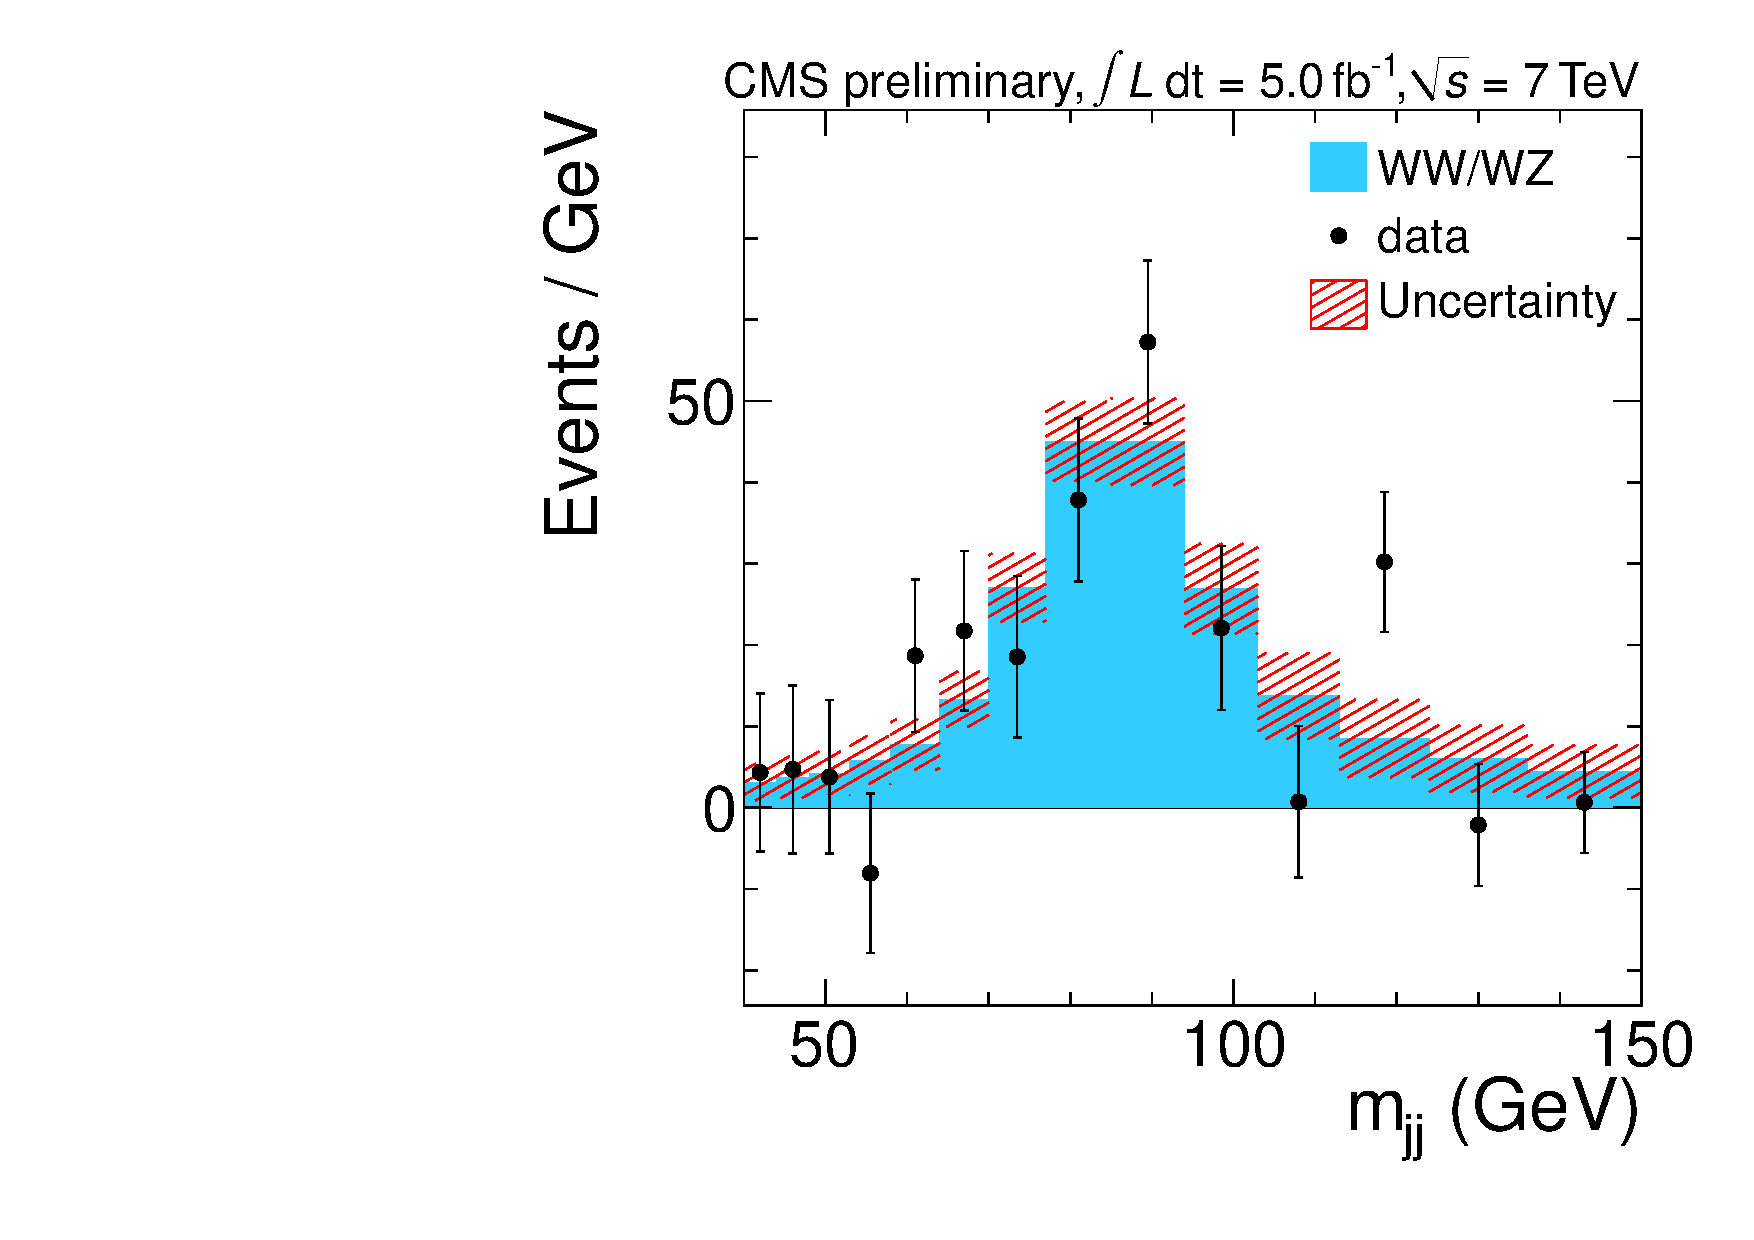
\includegraphics[width=0.49\textwidth]{figs/ScaleAndMatchingCrossChecks/mu2JNoBTag_fSU0fMU0/Wjj_Diboson_Muon_2jets_Subtracted.pdf}
    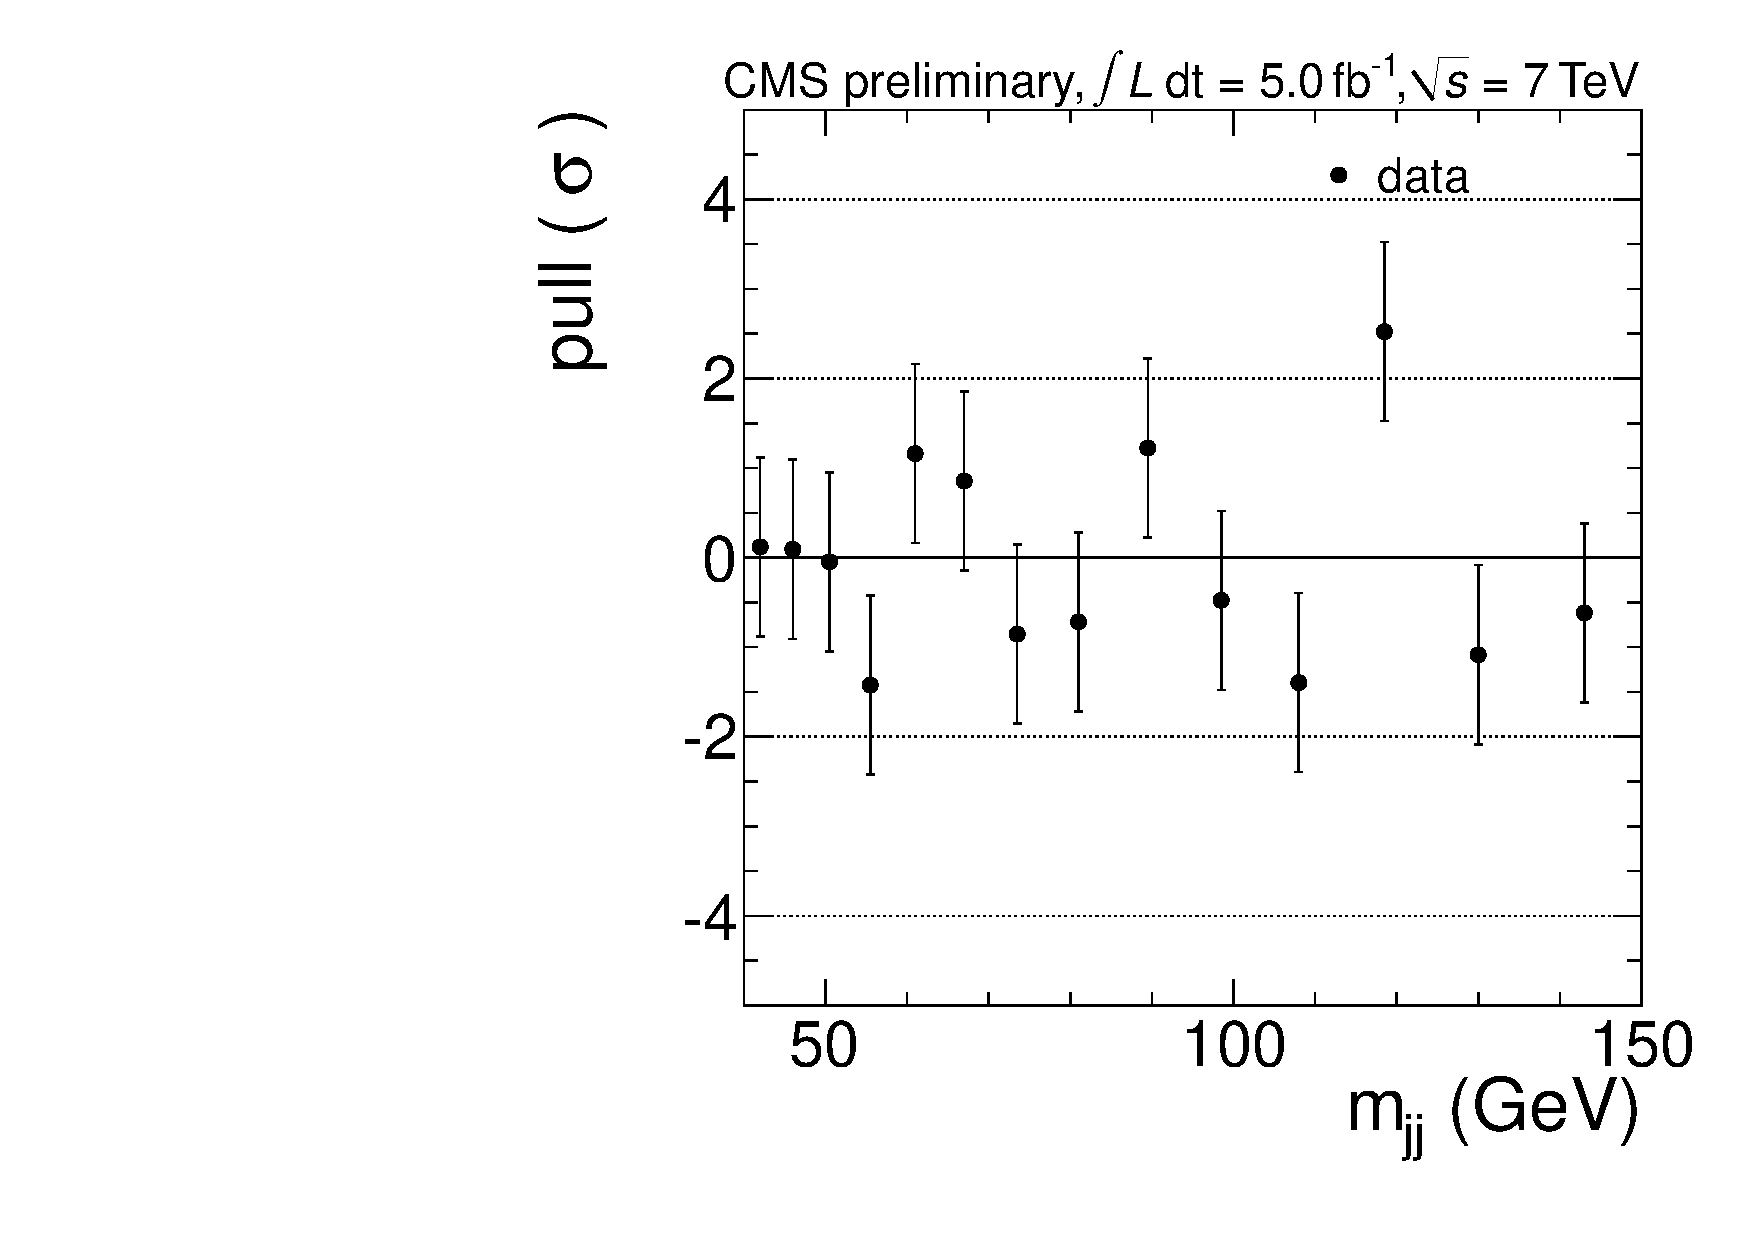
\includegraphics[width=0.49\textwidth]{figs/ScaleAndMatchingCrossChecks/mu2JNoBTag_fSU0fMU0/Wjj_Diboson_Muon_2jets_Pull.pdf}
    \caption{Distribution of the dijet invariant mass for the non-b-tagged 2-jet events in muon data and Monte Carlo with $f_{MU}=0$, $f_{SU}=0$: 
      (upper left) All background components stacked together, 
      (upper right) unstacked, (lower left) [Data minus all backgrounds except diboson],  
      (lower right) normalized residual between data and MC. }
    \label{fig:fsufmuXcheck_fSU0fMU0}}
\end{figure}
%%%%%%%%%%%%%%%%%%%%
%%%%%%%%%%%%%%%%%%%%
\begin{figure}[h!]
  {\centering
    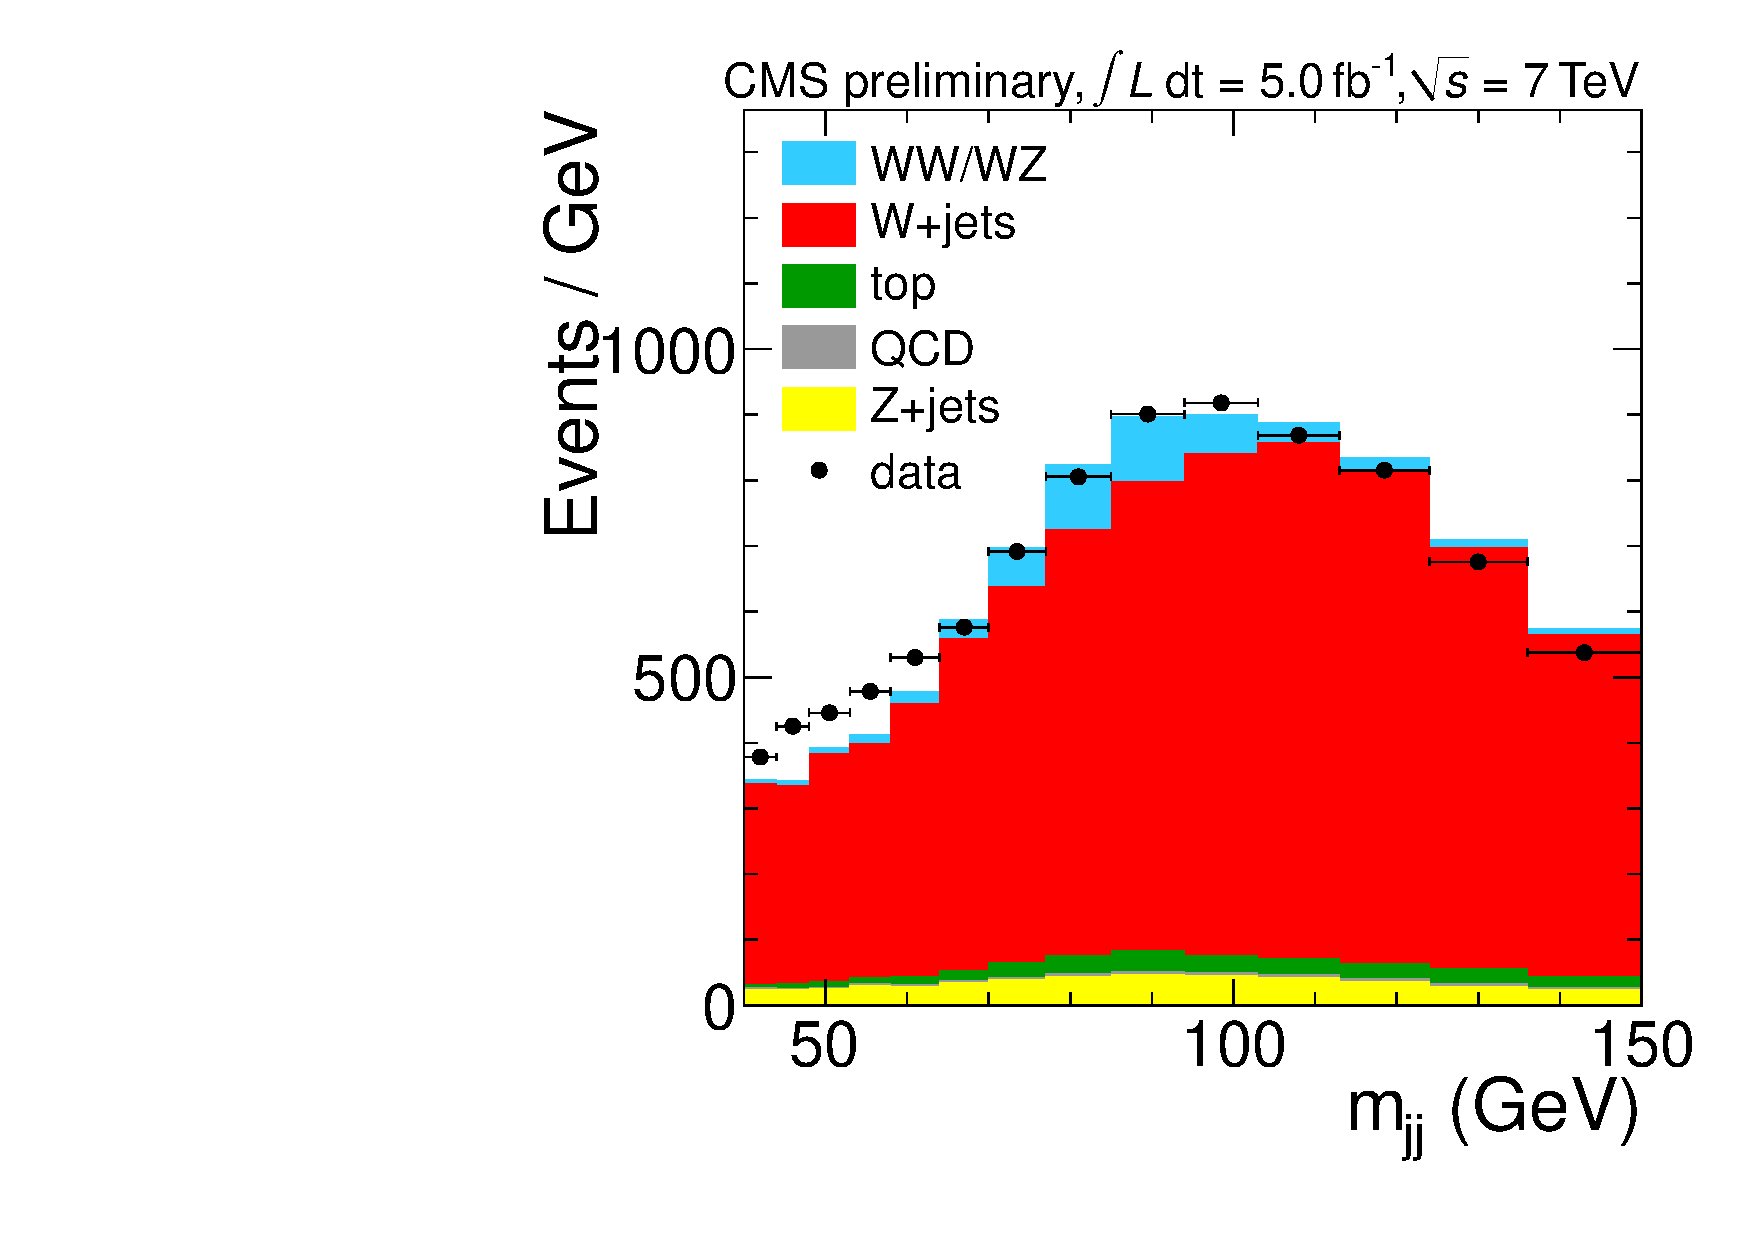
\includegraphics[width=0.49\textwidth]{figs/ScaleAndMatchingCrossChecks/mu2JNoBTag_fSUm1fMU0/Wjj_Diboson_Muon_2jets_Stacked.pdf}
    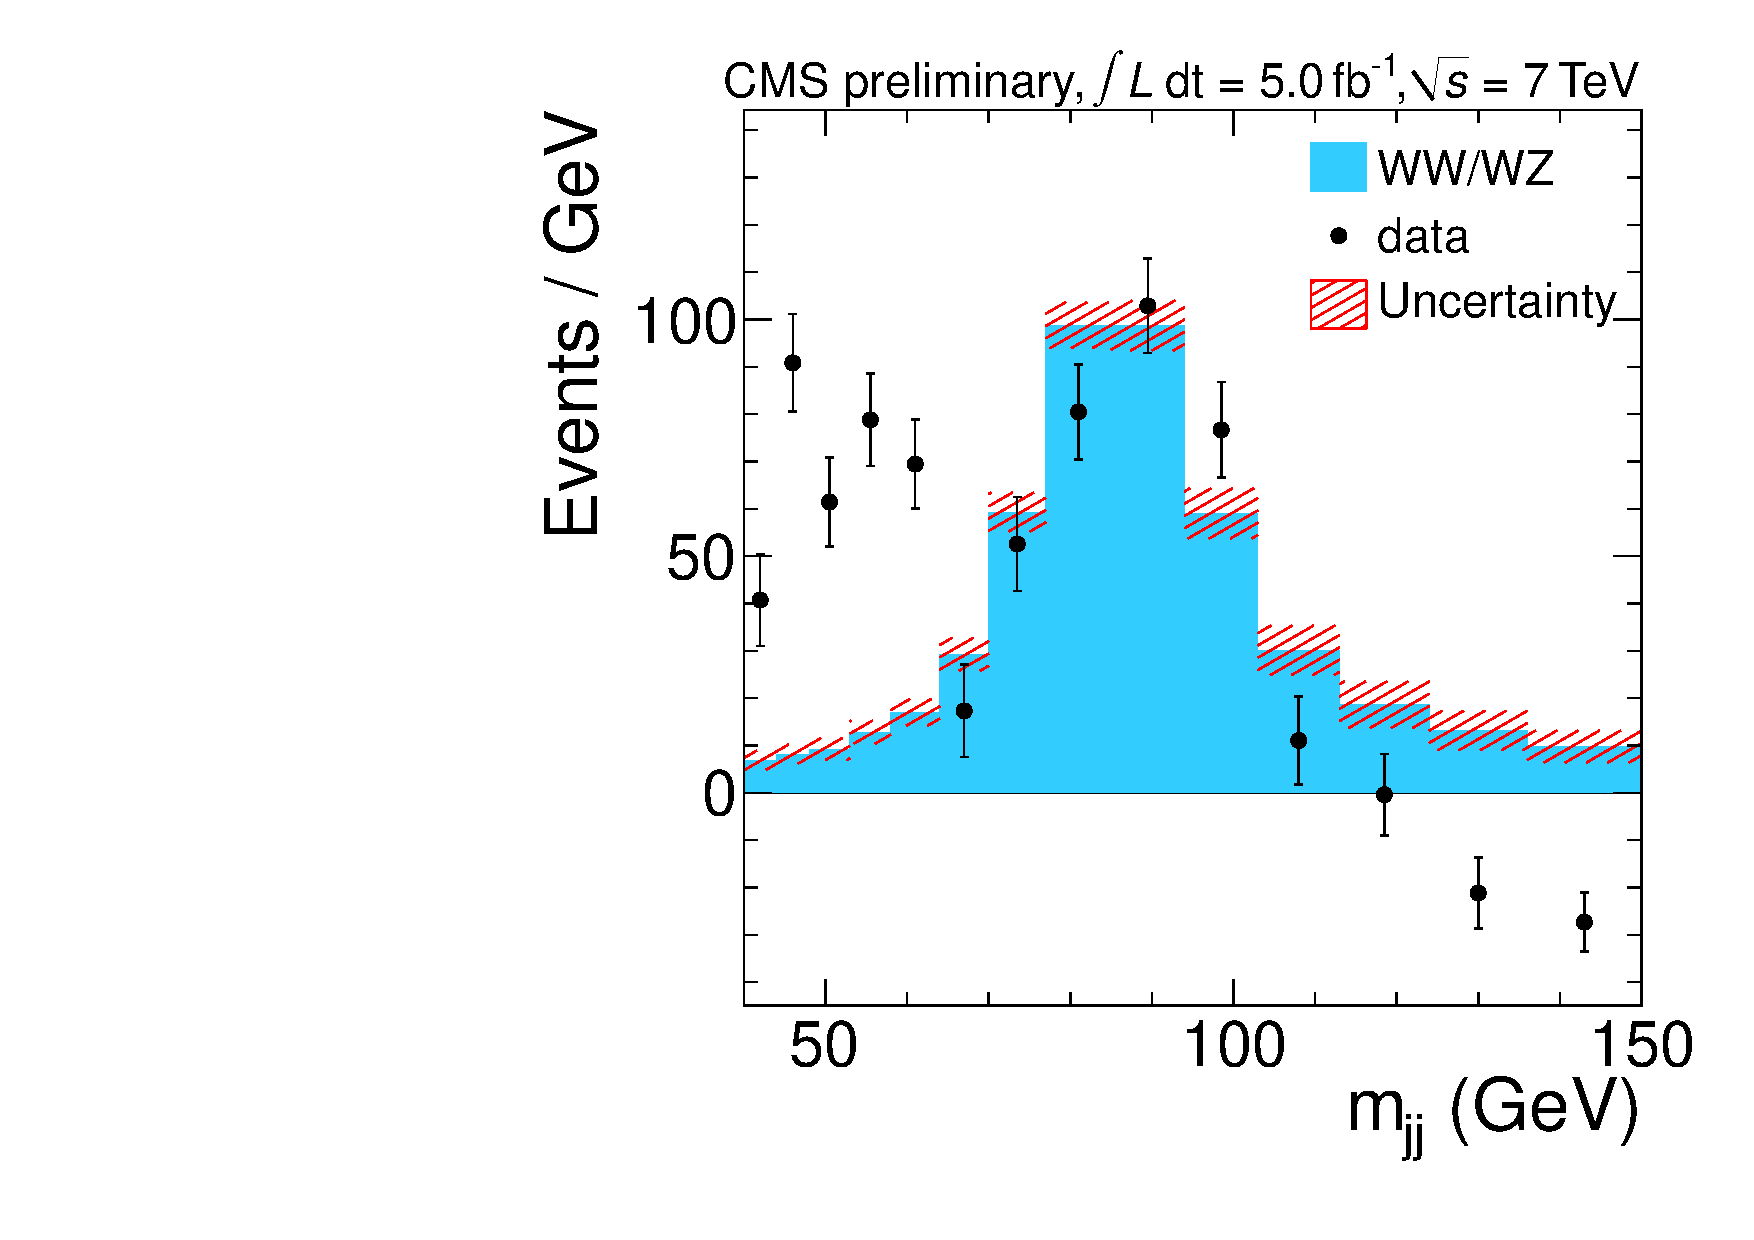
\includegraphics[width=0.49\textwidth]{figs/ScaleAndMatchingCrossChecks/mu2JNoBTag_fSUm1fMU0/Wjj_Diboson_Muon_2jets_Subtracted.pdf}
    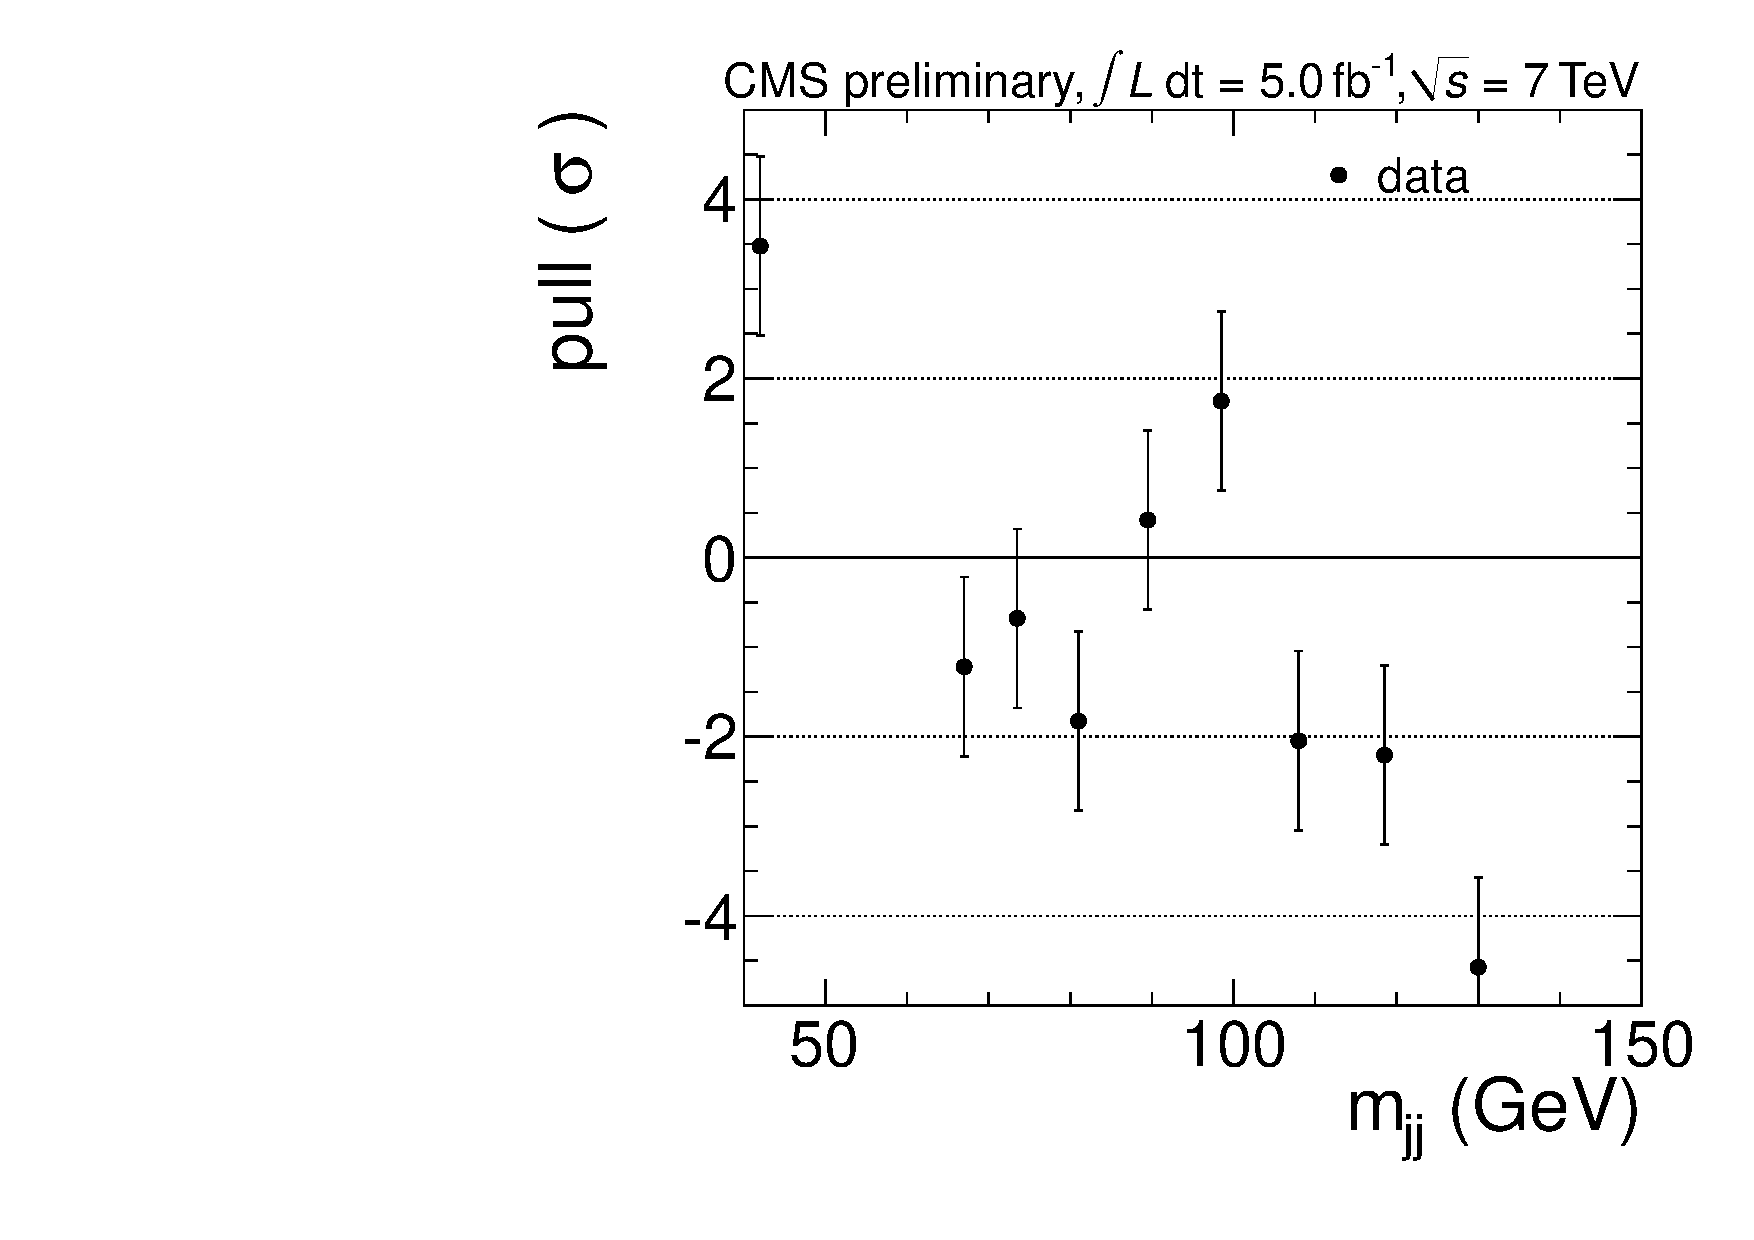
\includegraphics[width=0.49\textwidth]{figs/ScaleAndMatchingCrossChecks/mu2JNoBTag_fSUm1fMU0/Wjj_Diboson_Muon_2jets_Pull.pdf}
    \caption{Distribution of the dijet invariant mass for the non-b-tagged 2-jet events in muon data and Monte Carlo with $f_{MU}=0$, $f_{SU}=-1$: 
      (upper left) All background components stacked together, 
      (upper right) unstacked, (lower left) [Data minus all backgrounds except diboson],  
      (lower right) normalized residual between data and MC. }
    \label{fig:fsufmuXcheck_fSUm1fMU0}}
\end{figure}
%%%%%%%%%%%%%%%%%%%%
%%%%%%%%%%%%%%%%%%%%
\begin{figure}[h!]
  {\centering
    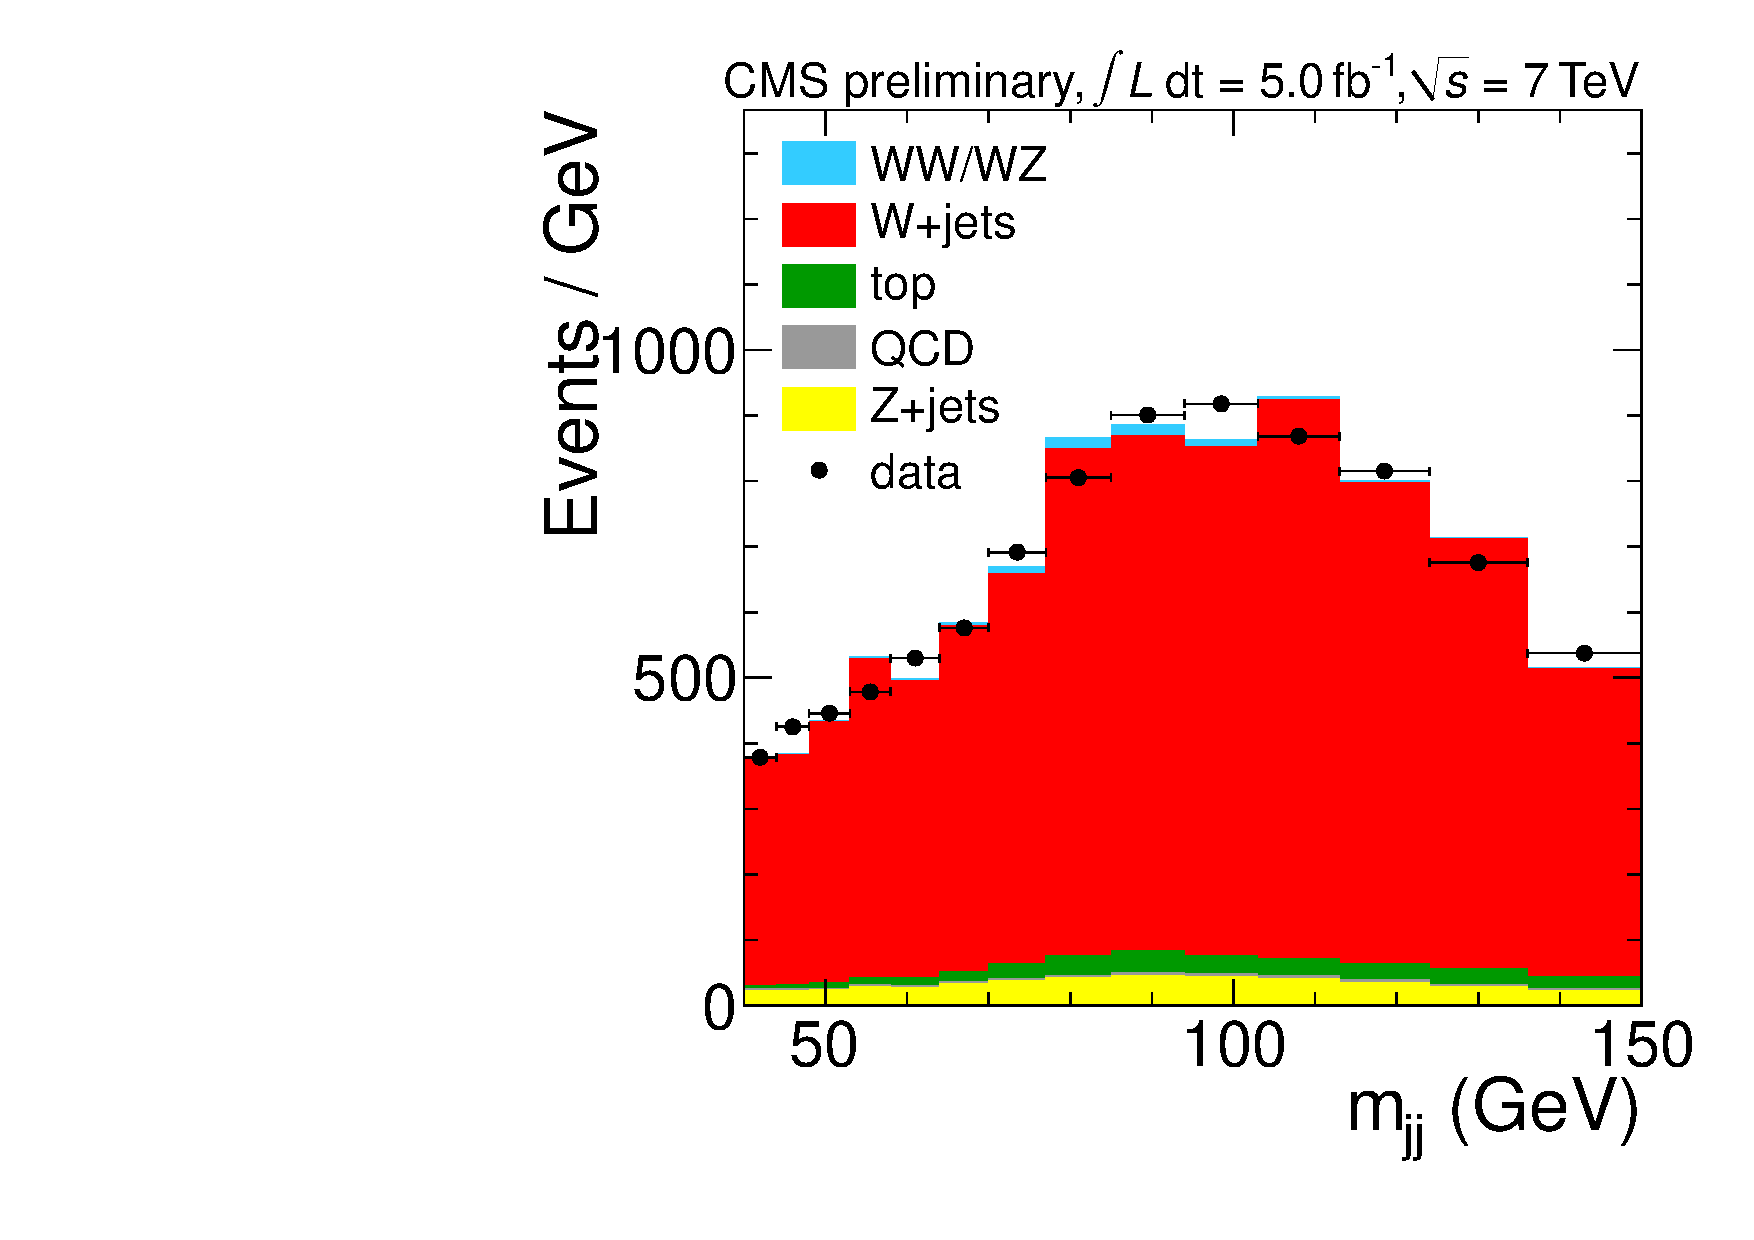
\includegraphics[width=0.49\textwidth]{figs/ScaleAndMatchingCrossChecks/mu2JNoBTag_fSUp1fMU0/Wjj_Diboson_Muon_2jets_Stacked.pdf}
    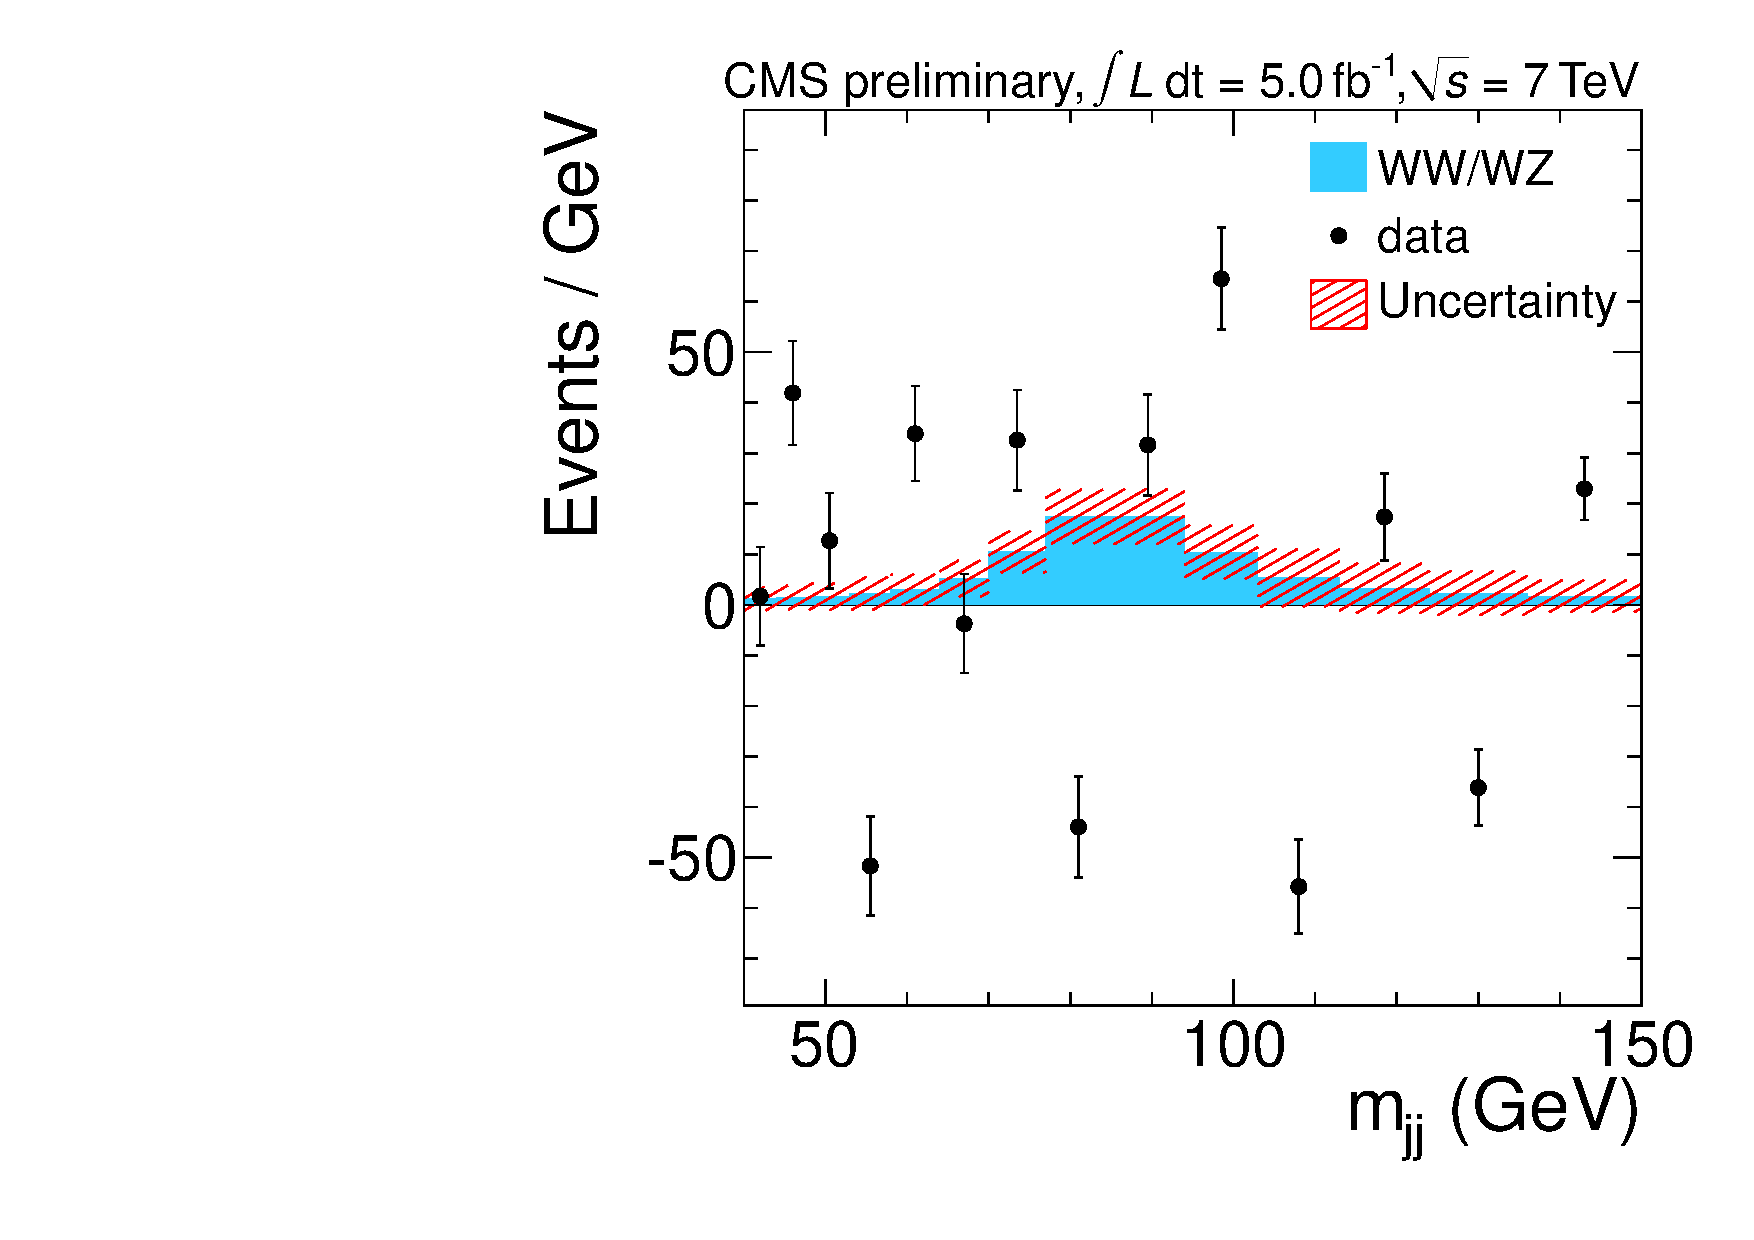
\includegraphics[width=0.49\textwidth]{figs/ScaleAndMatchingCrossChecks/mu2JNoBTag_fSUp1fMU0/Wjj_Diboson_Muon_2jets_Subtracted.pdf}
    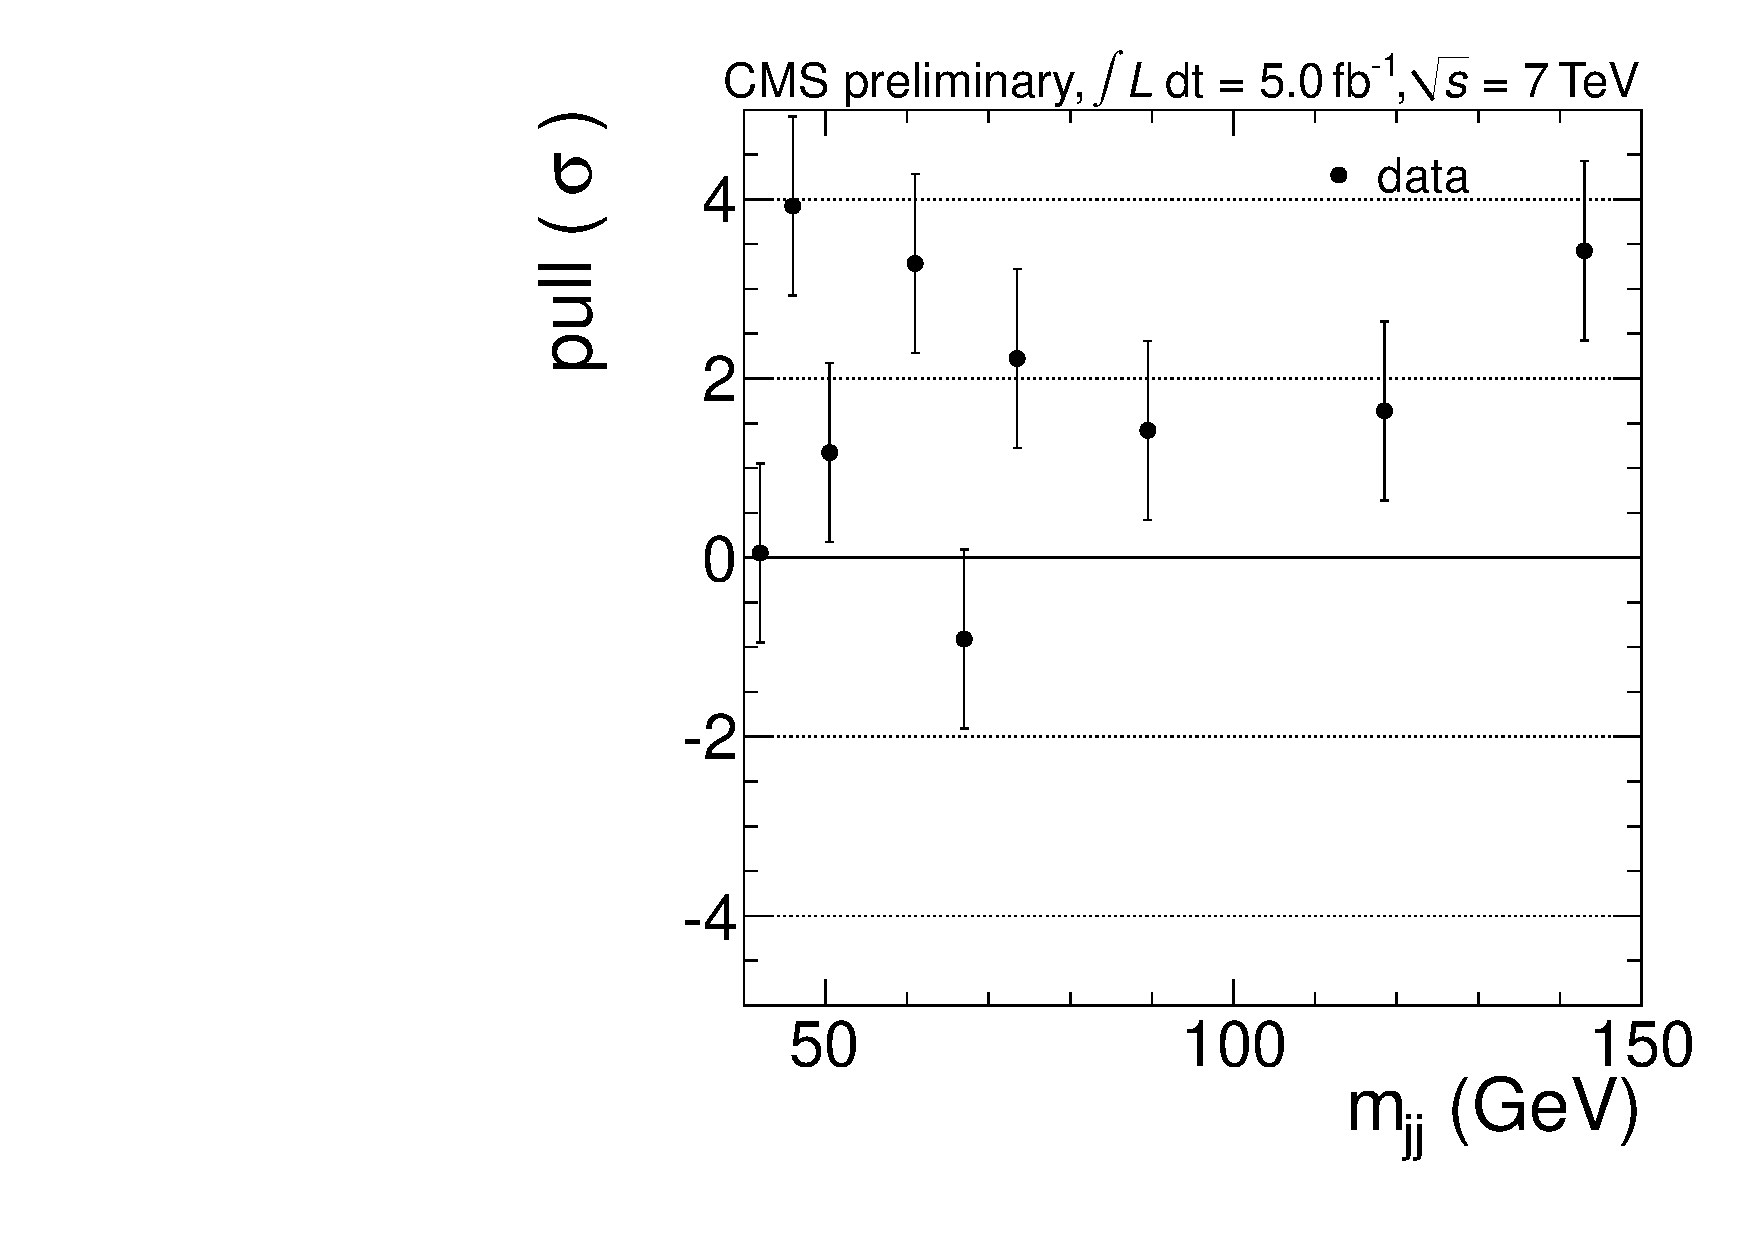
\includegraphics[width=0.49\textwidth]{figs/ScaleAndMatchingCrossChecks/mu2JNoBTag_fSUp1fMU0/Wjj_Diboson_Muon_2jets_Pull.pdf}
    \caption{Distribution of the dijet invariant mass for the non-b-tagged 2-jet events in muon data and Monte Carlo with $f_{MU}=0$, $f_{SU}=+1$: 
      (upper left) All background components stacked together, 
      (upper right) unstacked, (lower left) [Data minus all backgrounds except diboson],  
      (lower right) normalized residual between data and MC. }
    \label{fig:fsufmuXcheck_fSUp1fMU0}}
\end{figure}
%%%%%%%%%%%%%%%%%%%%
%%%%%%%%%%%%%%%%%%%%
\begin{figure}[h!]
  {\centering
    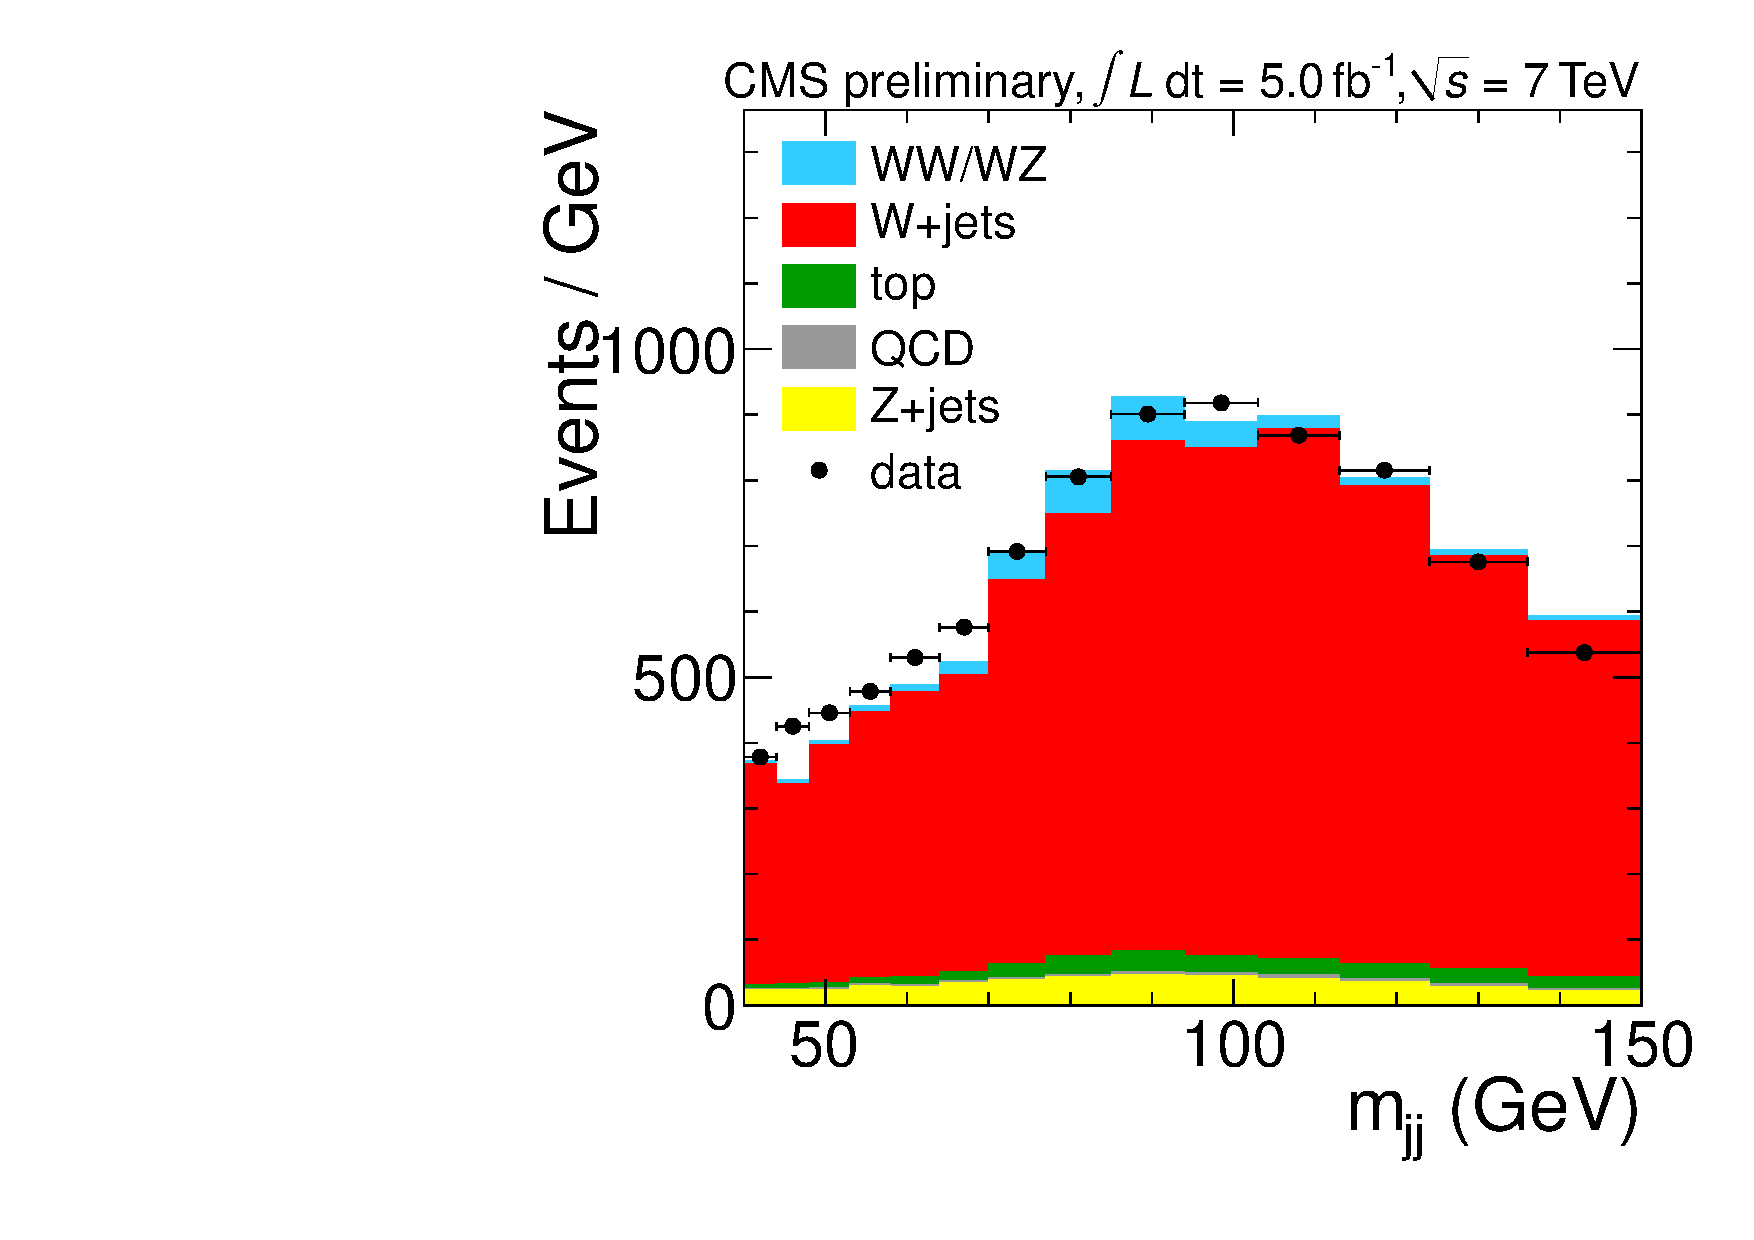
\includegraphics[width=0.49\textwidth]{figs/ScaleAndMatchingCrossChecks/mu2JNoBTag_fSU0fMUm1/Wjj_Diboson_Muon_2jets_Stacked.pdf}
    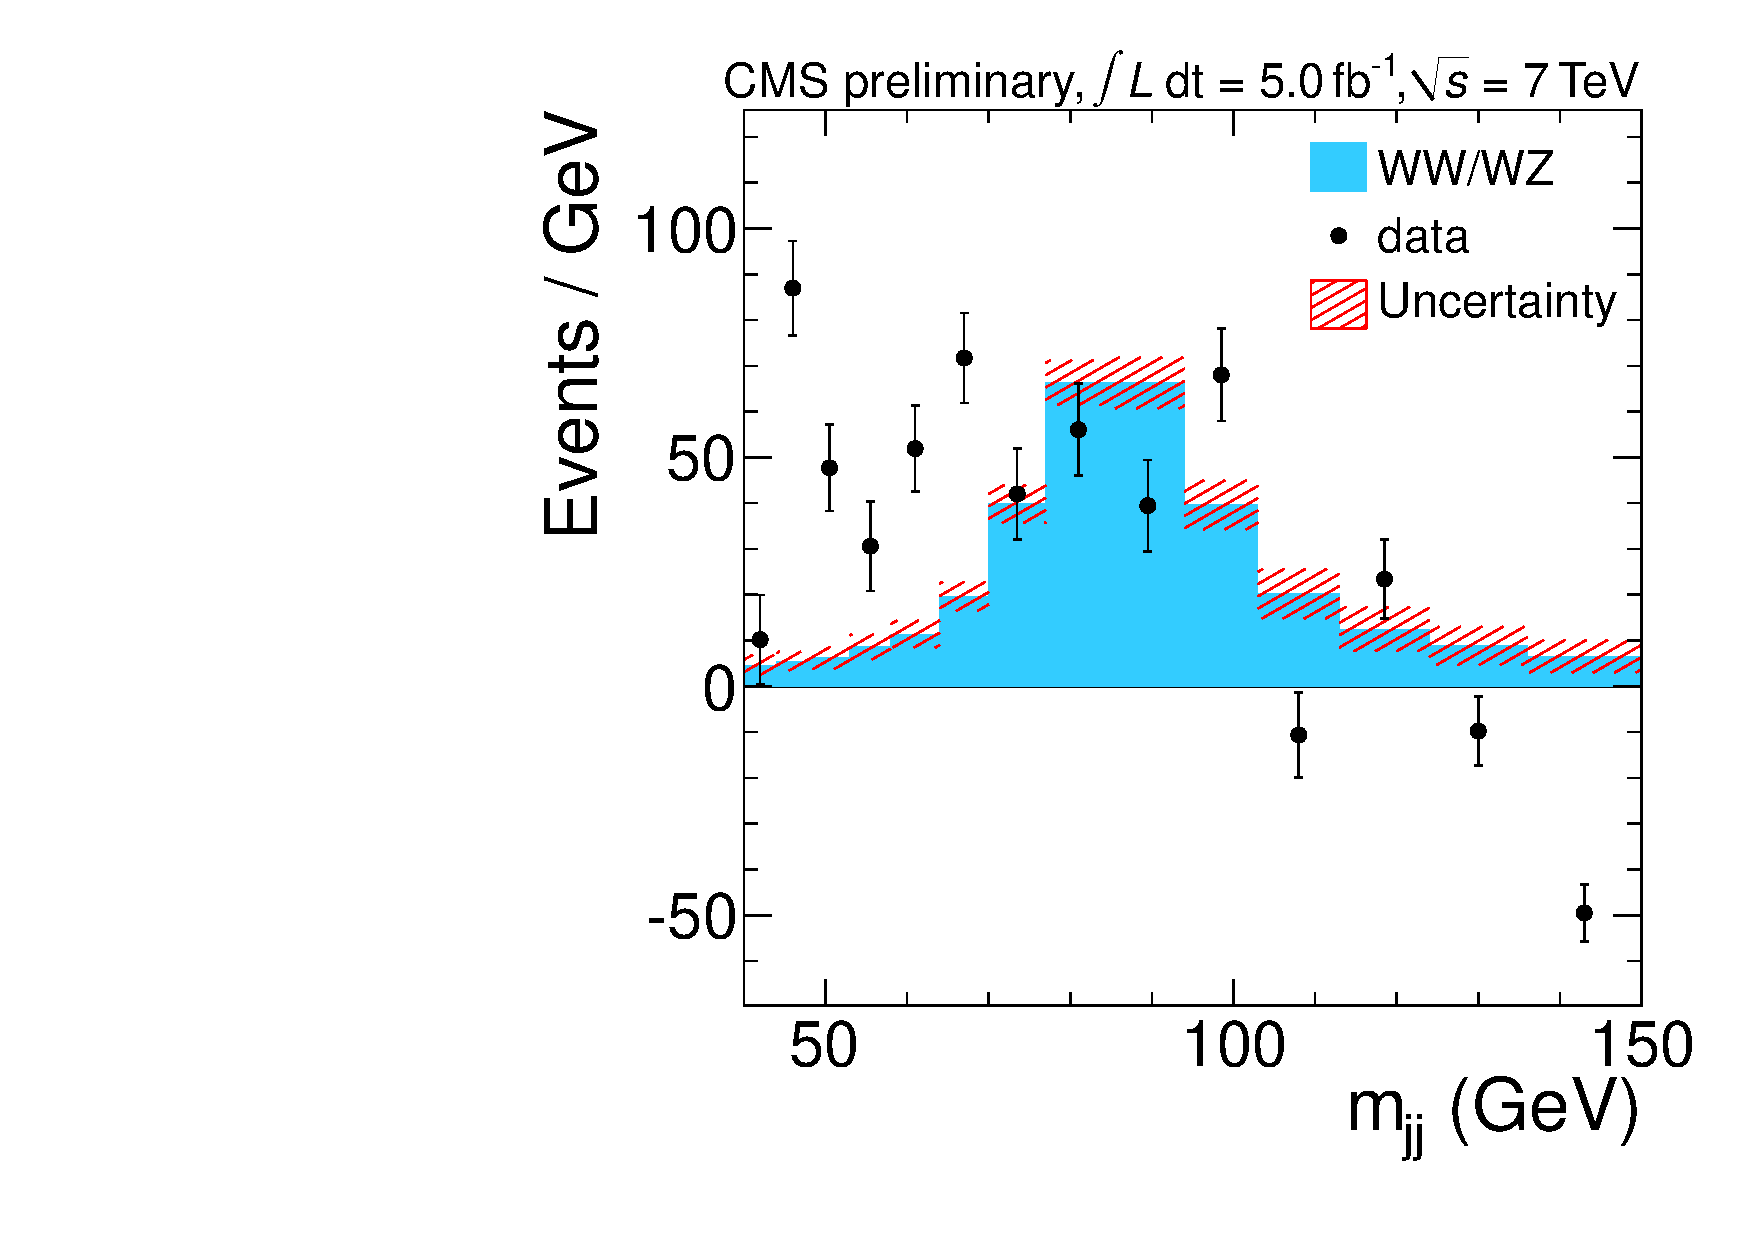
\includegraphics[width=0.49\textwidth]{figs/ScaleAndMatchingCrossChecks/mu2JNoBTag_fSU0fMUm1/Wjj_Diboson_Muon_2jets_Subtracted.pdf}
    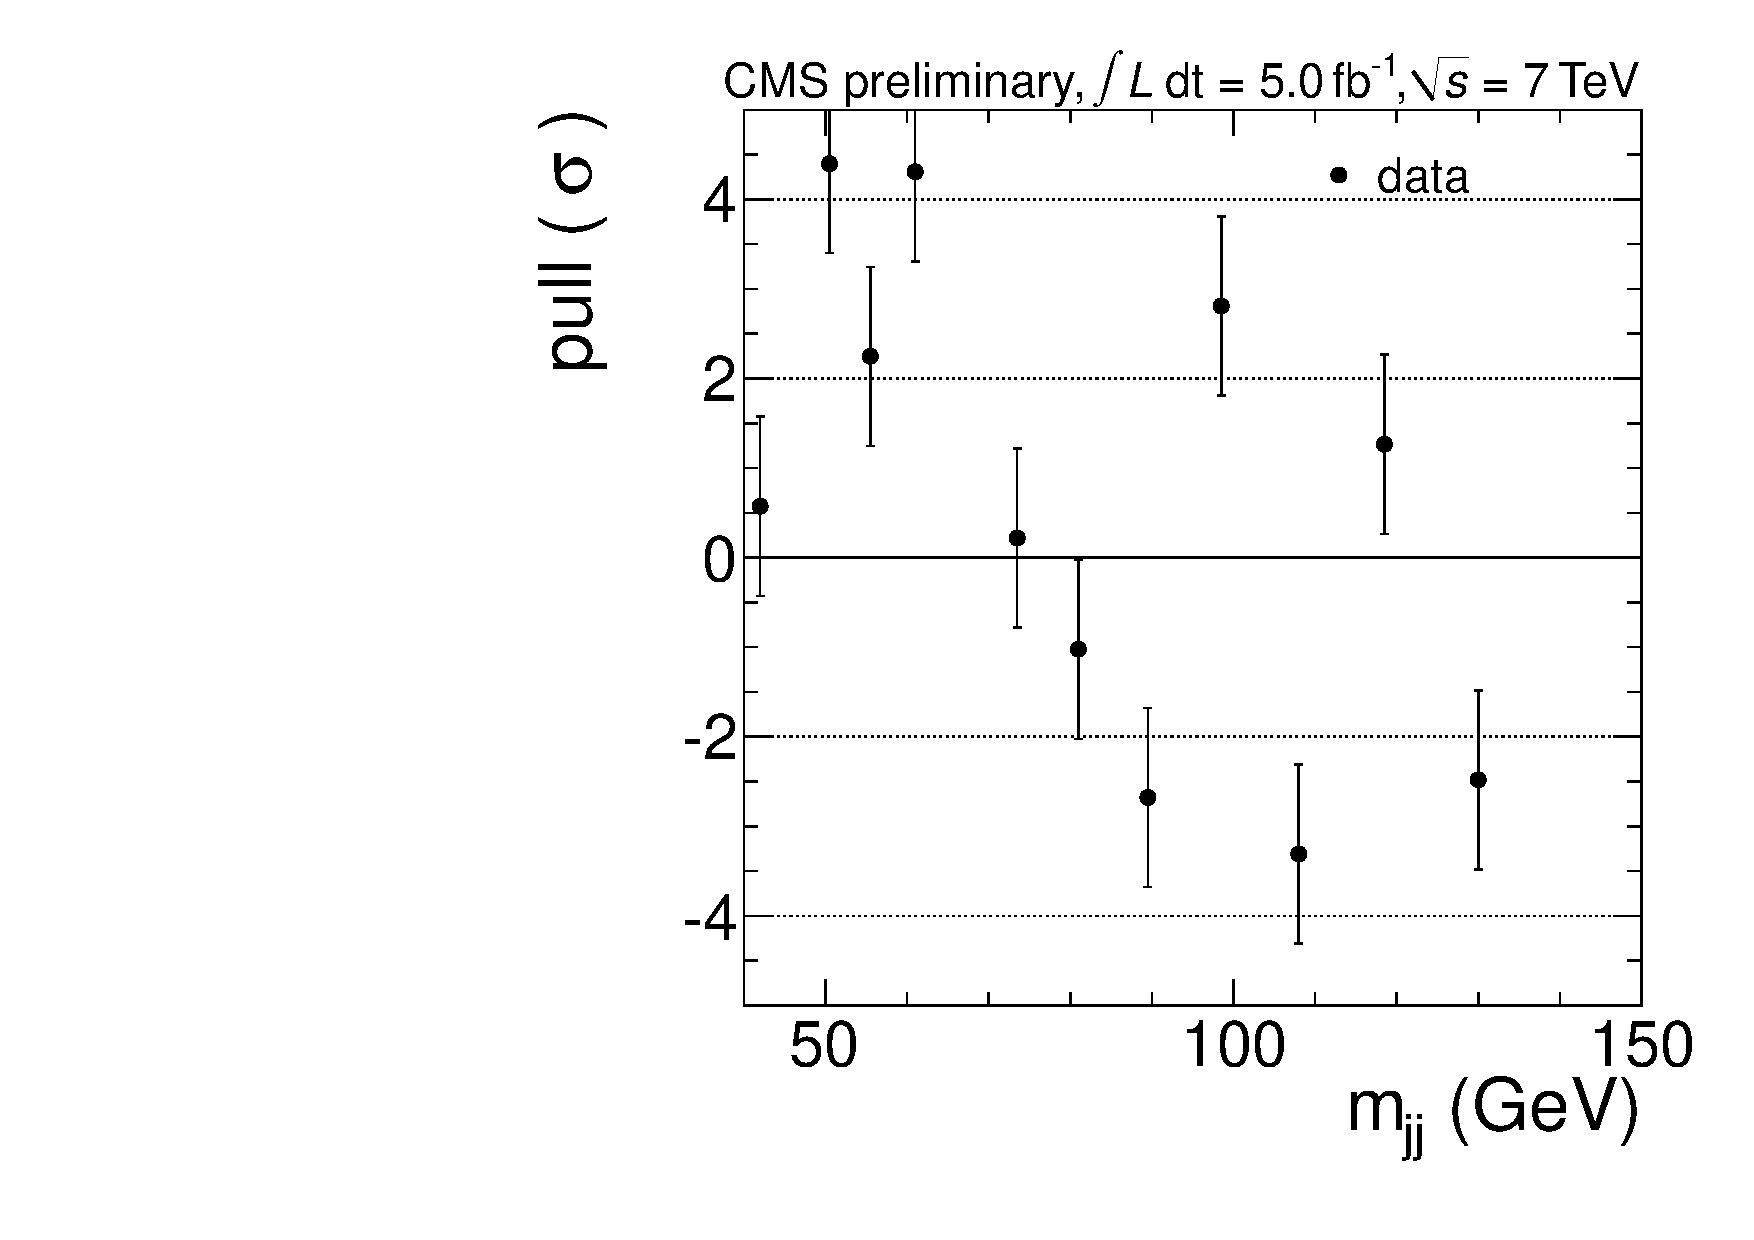
\includegraphics[width=0.49\textwidth]{figs/ScaleAndMatchingCrossChecks/mu2JNoBTag_fSU0fMUm1/Wjj_Diboson_Muon_2jets_Pull.pdf}
    \caption{Distribution of the dijet invariant mass for the non-b-tagged 2-jet events in muon data and Monte Carlo with $f_{MU}=-1$, $f_{SU}=0$: 
      (upper left) All background components stacked together, 
      (upper right) unstacked, (lower left) [Data minus all backgrounds except diboson],  
      (lower right) normalized residual between data and MC. }
    \label{fig:fsufmuXcheck_fSU0fMUm1}}
\end{figure}
%%%%%%%%%%%%%%%%%%%%
%%%%%%%%%%%%%%%%%%%%
\begin{figure}[h!]
  {\centering
    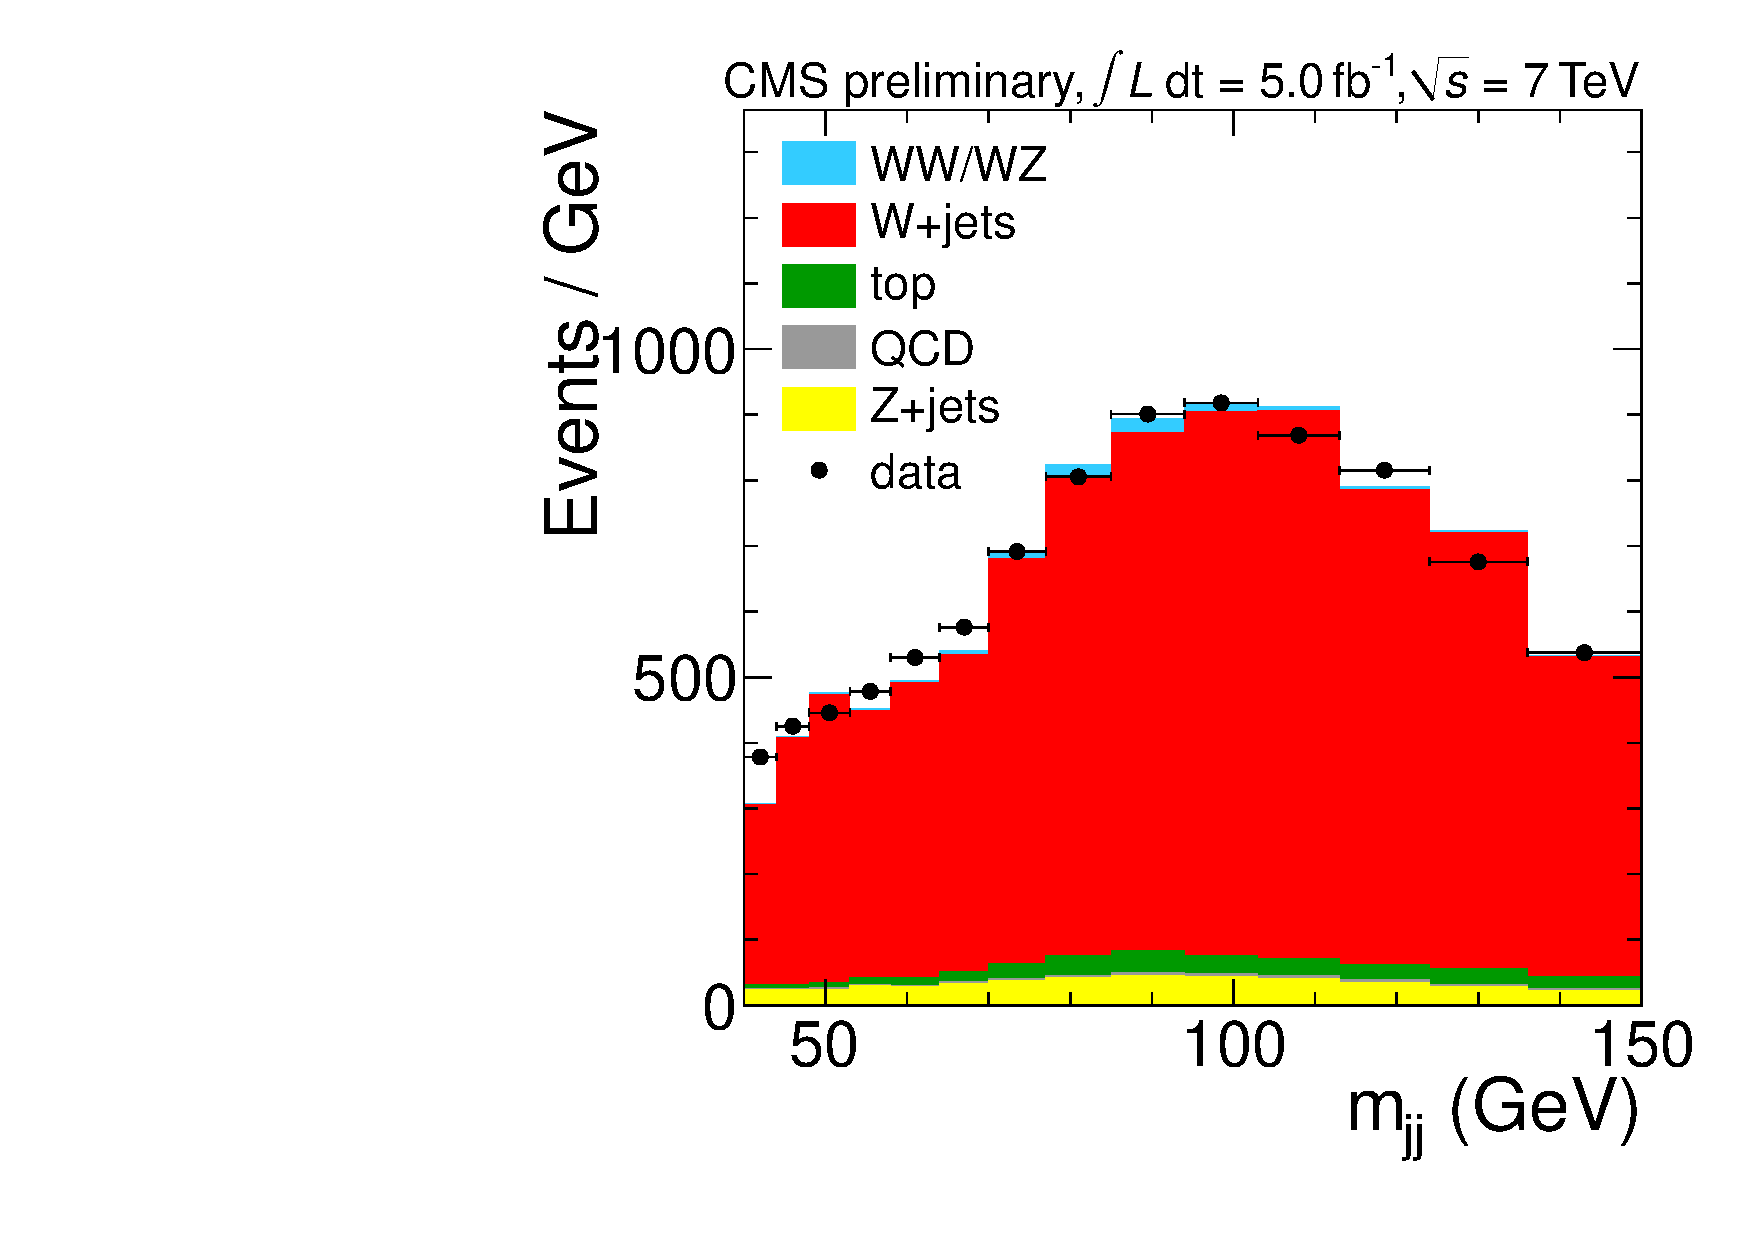
\includegraphics[width=0.49\textwidth]{figs/ScaleAndMatchingCrossChecks/mu2JNoBTag_fSU0fMUp1/Wjj_Diboson_Muon_2jets_Stacked.pdf}
    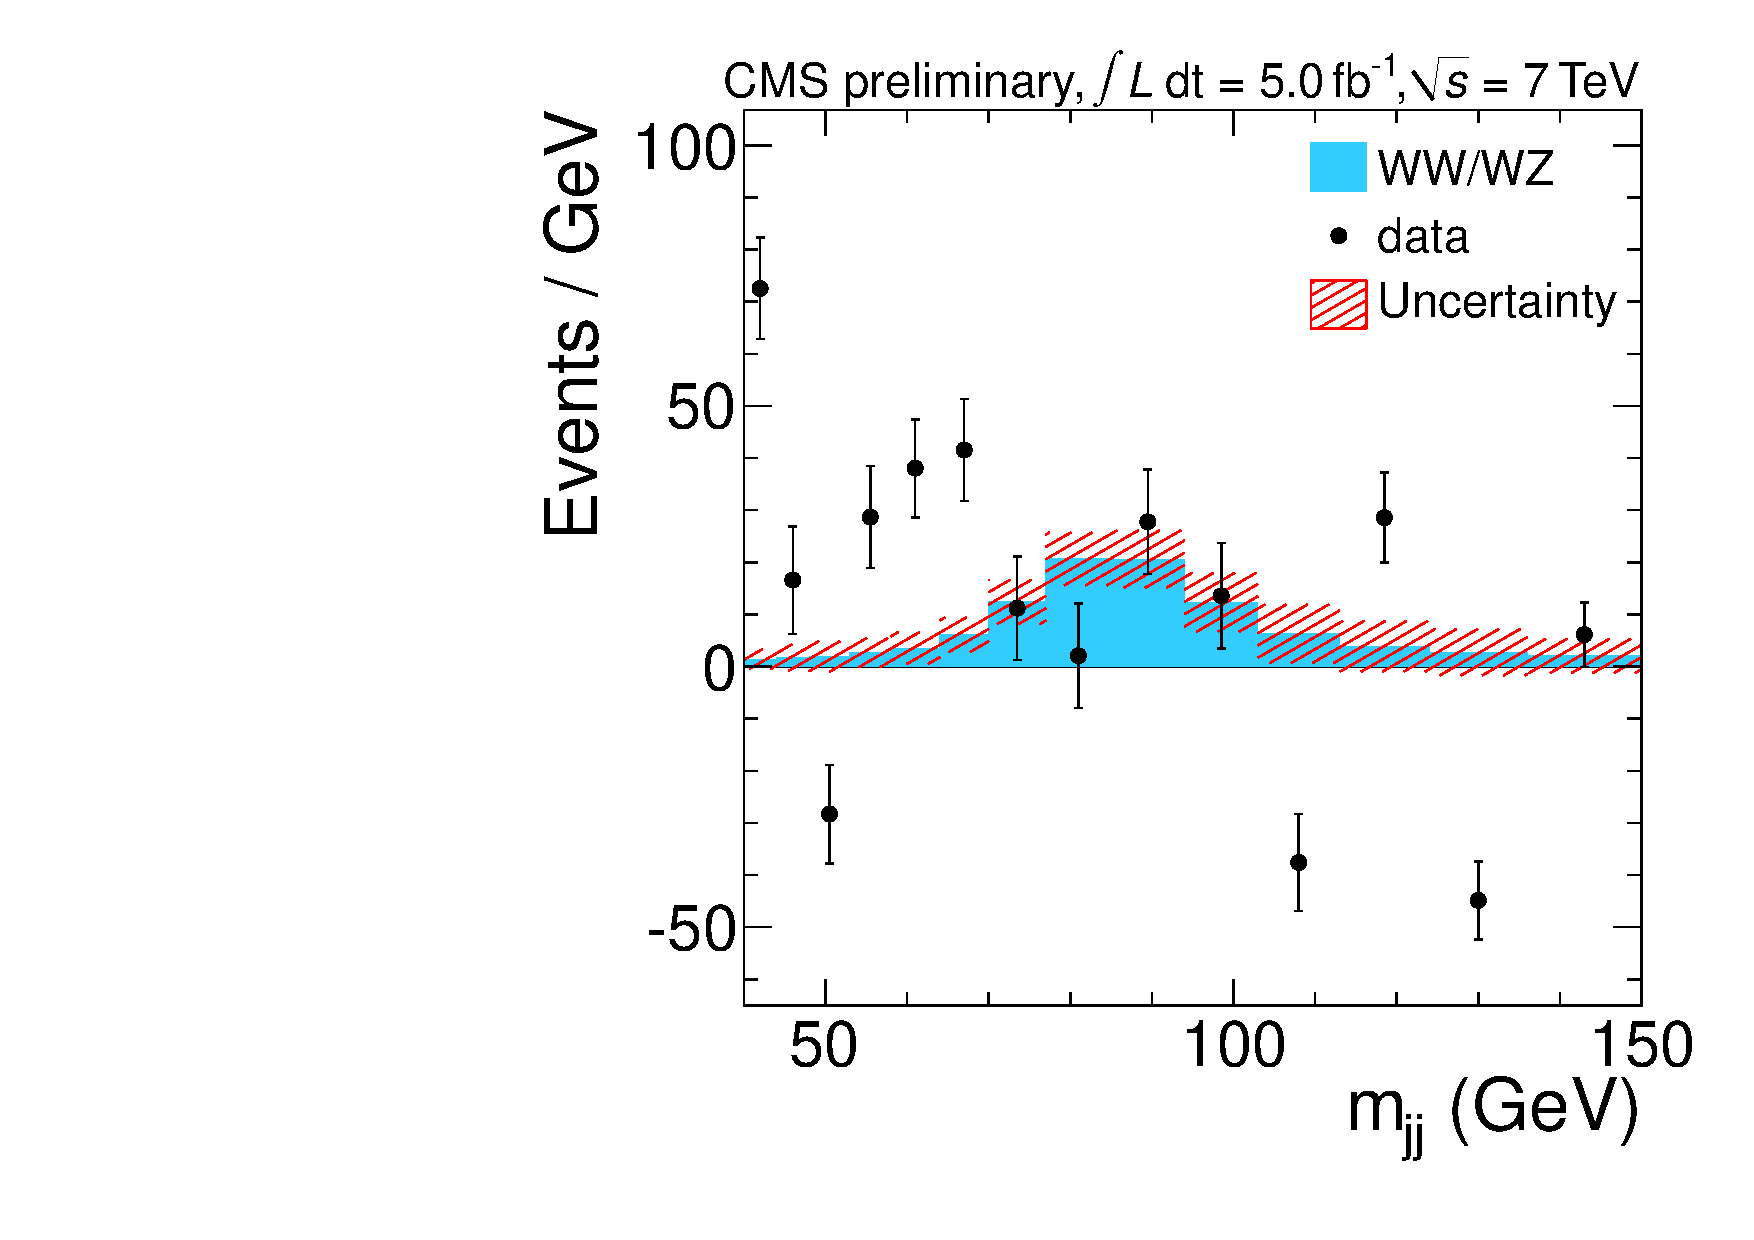
\includegraphics[width=0.49\textwidth]{figs/ScaleAndMatchingCrossChecks/mu2JNoBTag_fSU0fMUp1/Wjj_Diboson_Muon_2jets_Subtracted.pdf}
    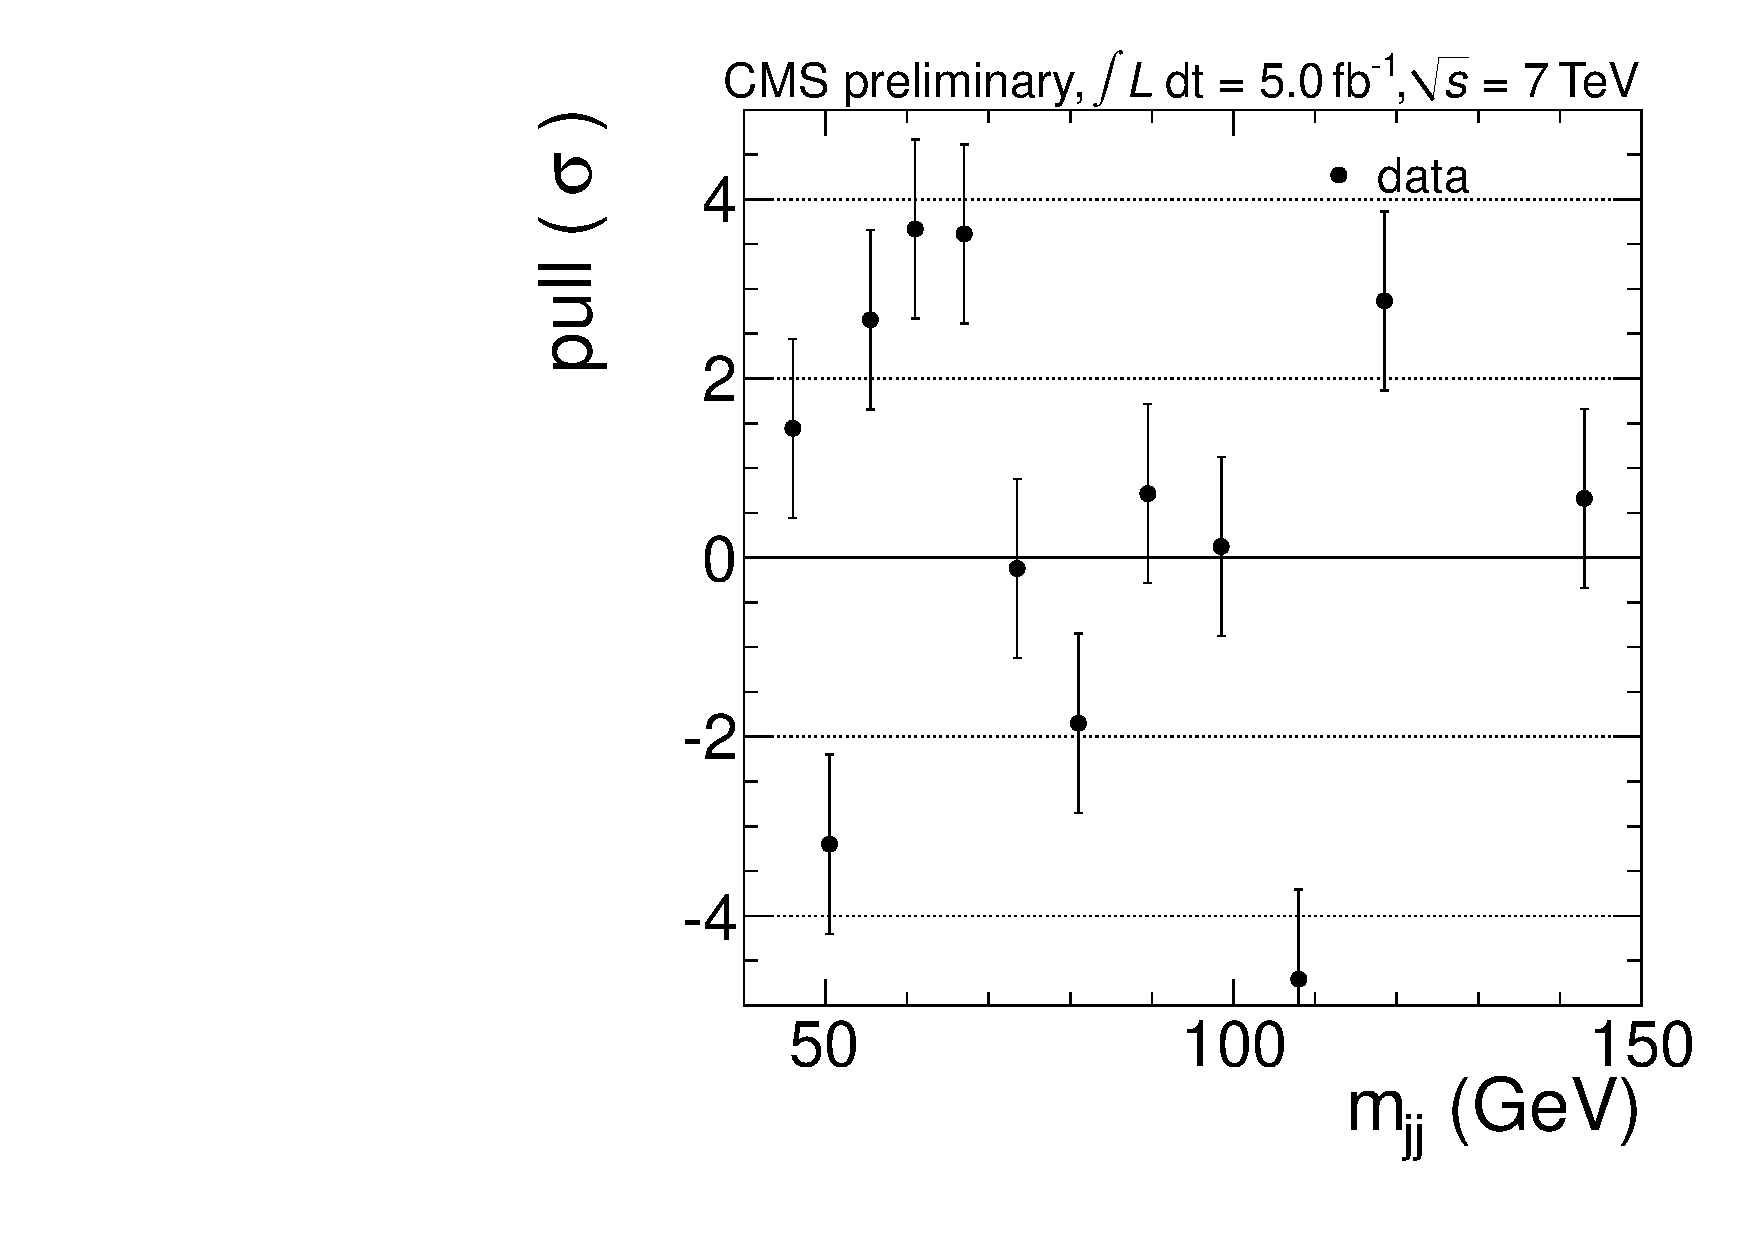
\includegraphics[width=0.49\textwidth]{figs/ScaleAndMatchingCrossChecks/mu2JNoBTag_fSU0fMUp1/Wjj_Diboson_Muon_2jets_Pull.pdf}
    \caption{Distribution of the dijet invariant mass for the non-b-tagged 2-jet events in muon data and Monte Carlo with $f_{MU}=+1$, $f_{SU}=0$: 
      (upper left) All background components stacked together, 
      (upper right) unstacked, (lower left) [Data minus all backgrounds except diboson],  
      (lower right) normalized residual between data and MC. }
    \label{fig:fsufmuXcheck_fSU0fMUp1}}
\end{figure}
%%%%%%%%%%%%%%%%%%%%
%%%%%%%%%%%%%%%%%%%%
\begin{figure}[h!]
  {\centering
    \includegraphics[width=0.49\textwidth]{figs/ScaleAndMatchingCrossChecks/mu2JNoBTag_fSUm1sigmafMUDef/Wjj_Diboson_Muon_2jets_Stacked.pdf}
    \includegraphics[width=0.49\textwidth]{figs/ScaleAndMatchingCrossChecks/mu2JNoBTag_fSUm1sigmafMUDef/Wjj_Diboson_Muon_2jets_Subtracted.pdf}
    \includegraphics[width=0.49\textwidth]{figs/ScaleAndMatchingCrossChecks/mu2JNoBTag_fSUm1sigmafMUDef/Wjj_Diboson_Muon_2jets_Pull.pdf}
    \caption{Distribution of the dijet invariant mass for the non-b-tagged 2-jet events in muon data and Monte Carlo with $f_{SU}$ changed by $-1\sigma$: 
      (upper left) All background components stacked together, 
      (upper right) unstacked, (lower left) [Data minus all backgrounds except diboson],  
      (lower right) normalized residual between data and MC. }
    \label{fig:fsufmuXcheck_fSUm1sigmafMUDef}}
\end{figure}
%%%%%%%%%%%%%%%%%%%%
%%%%%%%%%%%%%%%%%%%%
\begin{figure}[h!]
  {\centering
    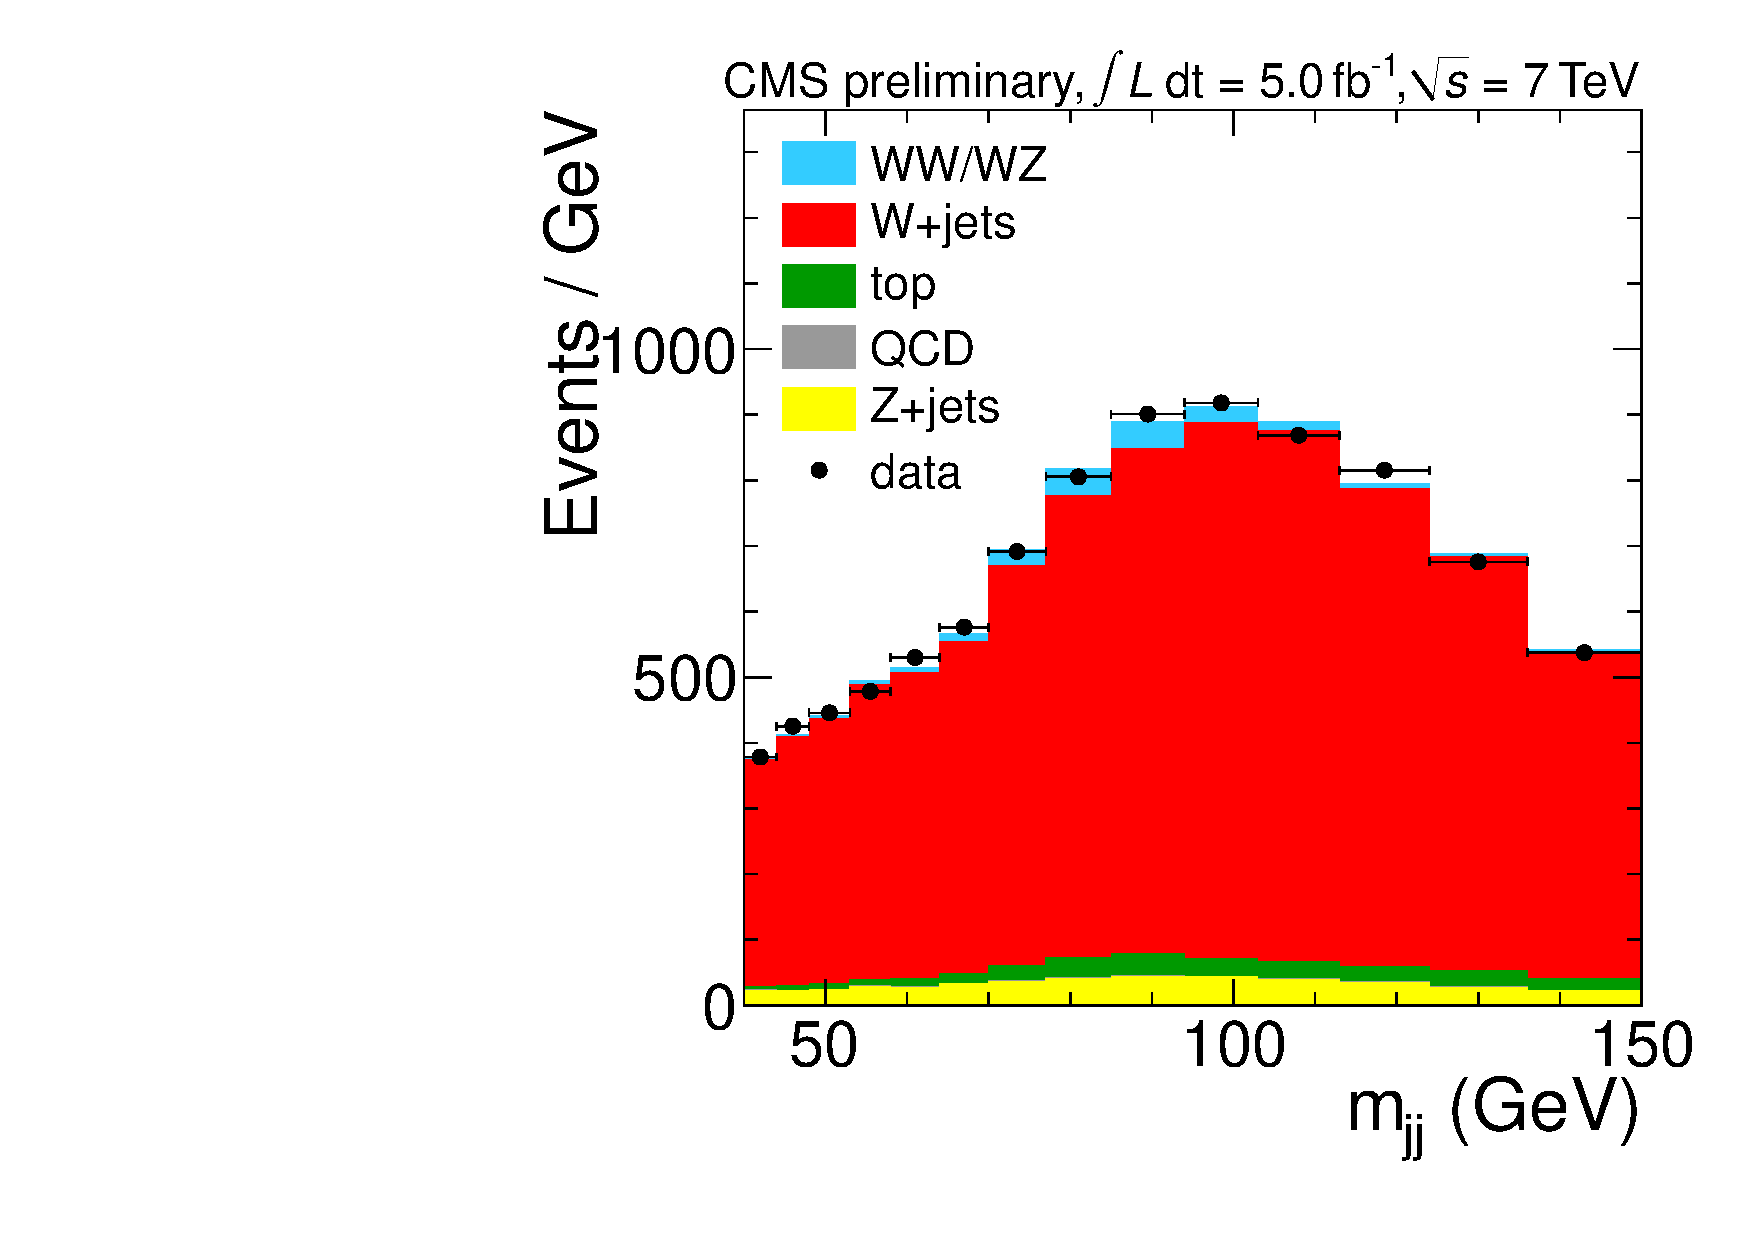
\includegraphics[width=0.49\textwidth]{figs/ScaleAndMatchingCrossChecks/mu2JNoBTag_fSUp1sigmafMUDef/Wjj_Diboson_Muon_2jets_Stacked.pdf}
    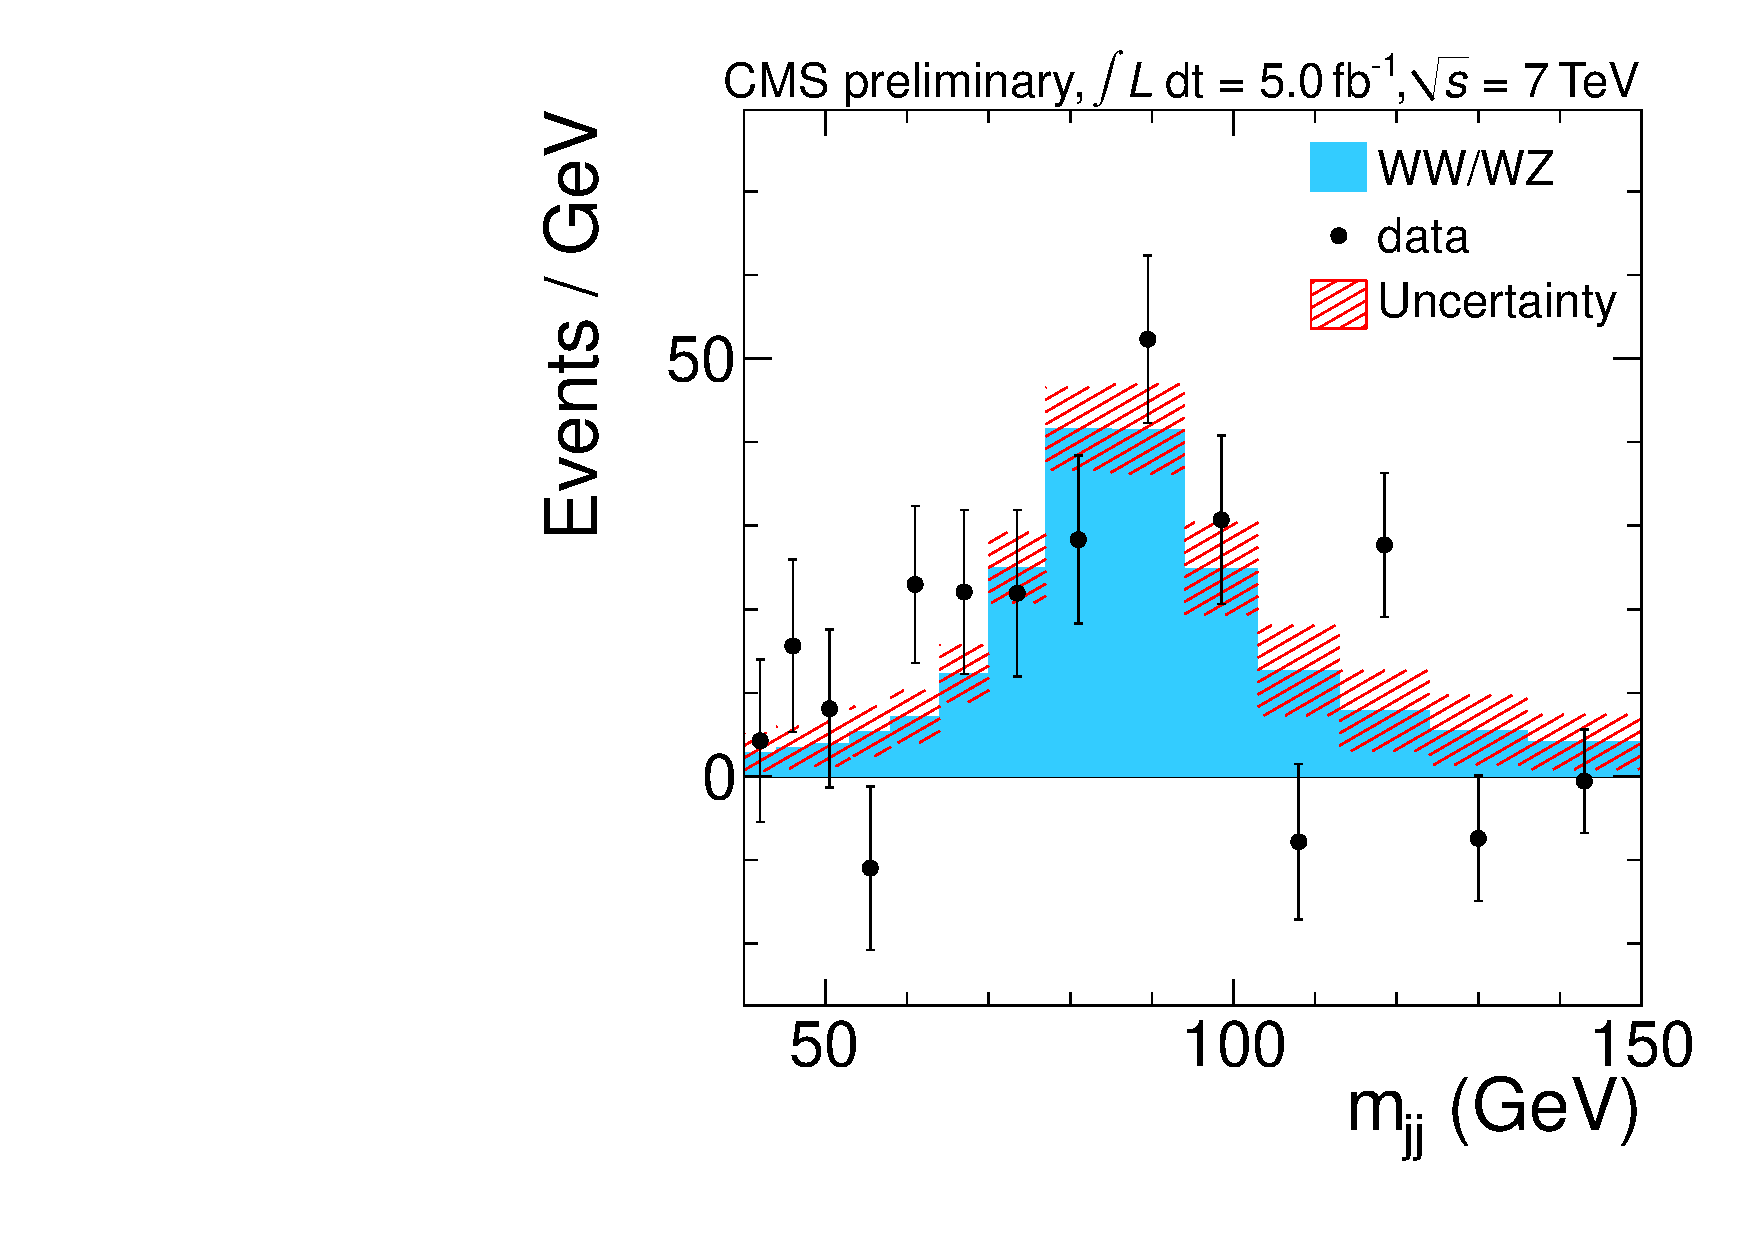
\includegraphics[width=0.49\textwidth]{figs/ScaleAndMatchingCrossChecks/mu2JNoBTag_fSUp1sigmafMUDef/Wjj_Diboson_Muon_2jets_Subtracted.pdf}
    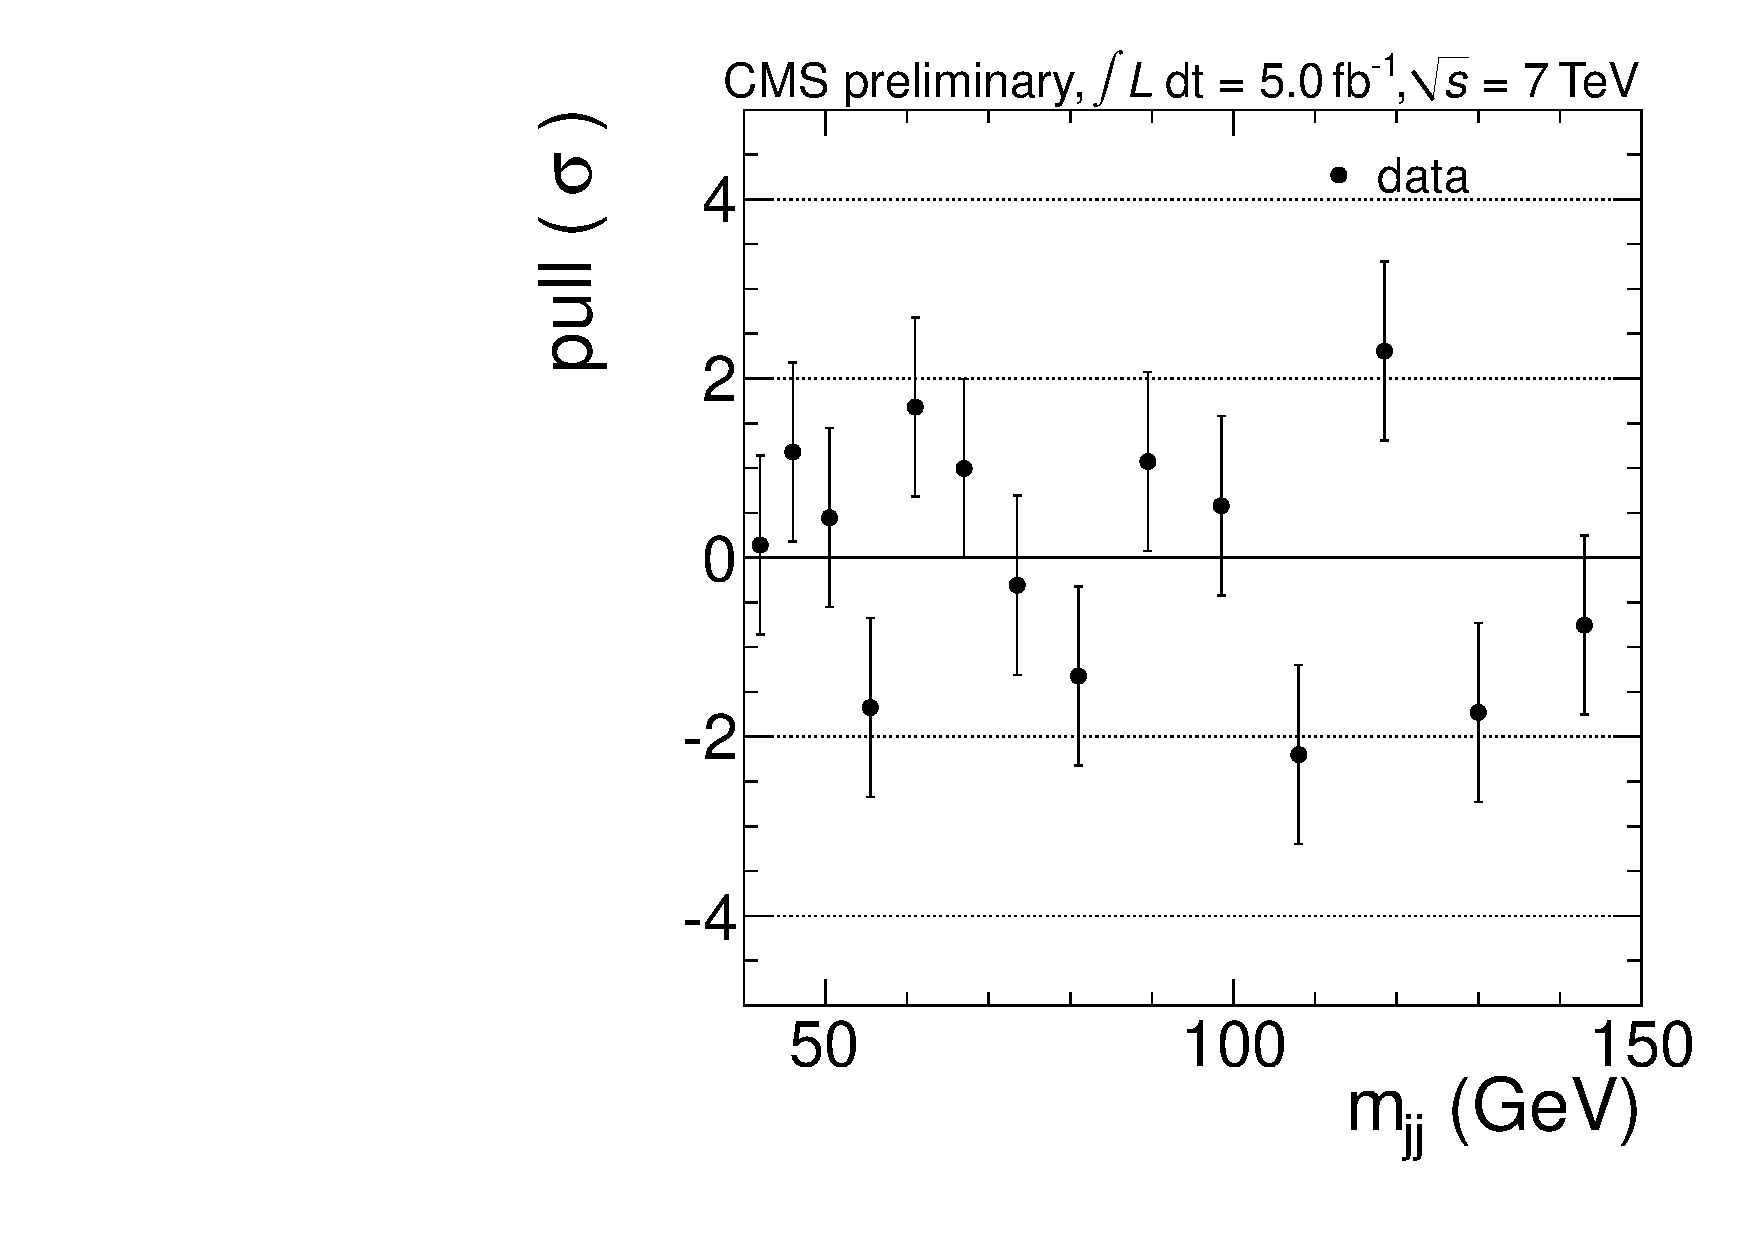
\includegraphics[width=0.49\textwidth]{figs/ScaleAndMatchingCrossChecks/mu2JNoBTag_fSUp1sigmafMUDef/Wjj_Diboson_Muon_2jets_Pull.pdf}
    \caption{Distribution of the dijet invariant mass for the non-b-tagged 2-jet events in muon data and Monte Carlo with $f_{SU}$ changed by $+1\sigma$: 
      (upper left) All background components stacked together, 
      (upper right) unstacked, (lower left) [Data minus all backgrounds except diboson],  
      (lower right) normalized residual between data and MC. }
    \label{fig:fsufmuXcheck_fSUp1sigmafMUDef}}
\end{figure}
%%%%%%%%%%%%%%%%%%%%
%%%%%%%%%%%%%%%%%%%%
\begin{figure}[h!]
  {\centering
    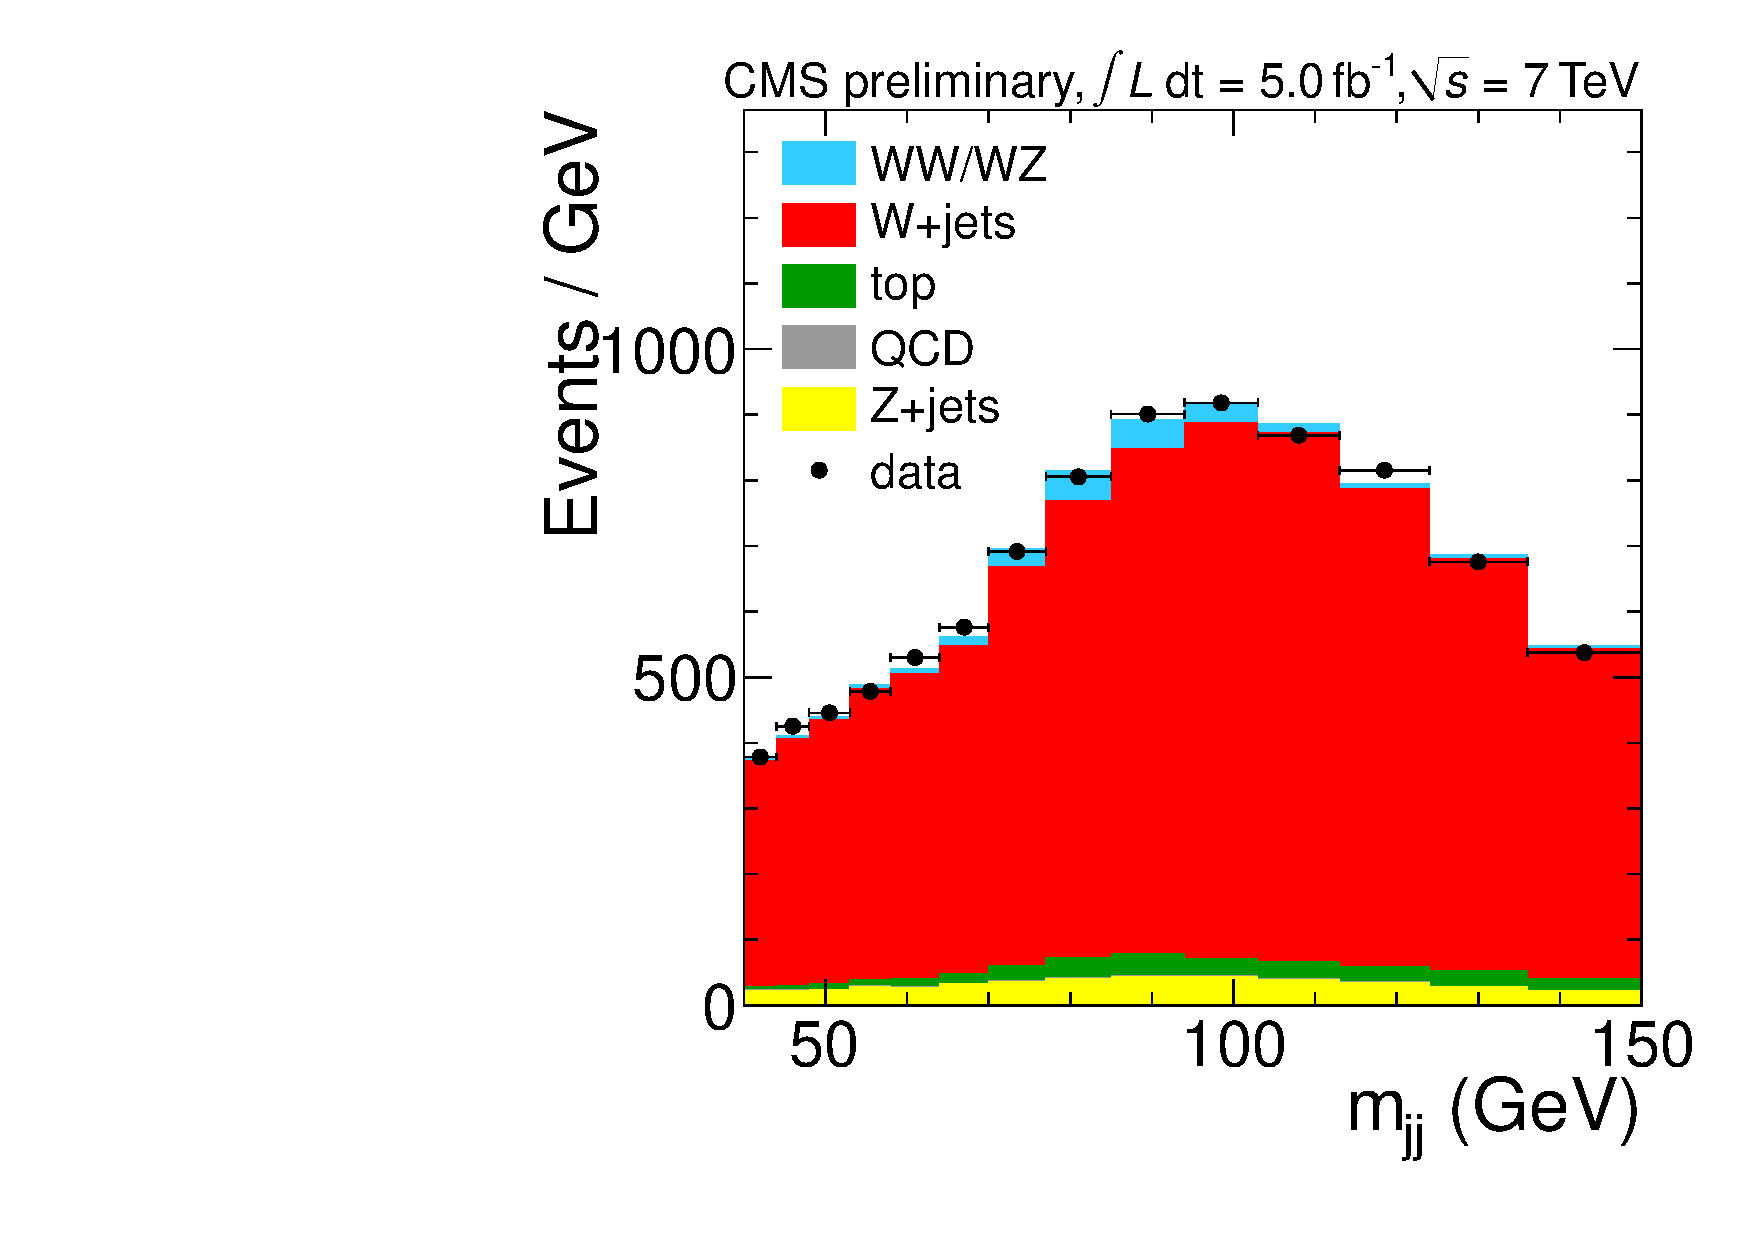
\includegraphics[width=0.49\textwidth]{figs/ScaleAndMatchingCrossChecks/mu2JNoBTag_fSUDeffMUm1sigma/Wjj_Diboson_Muon_2jets_Stacked.pdf}
    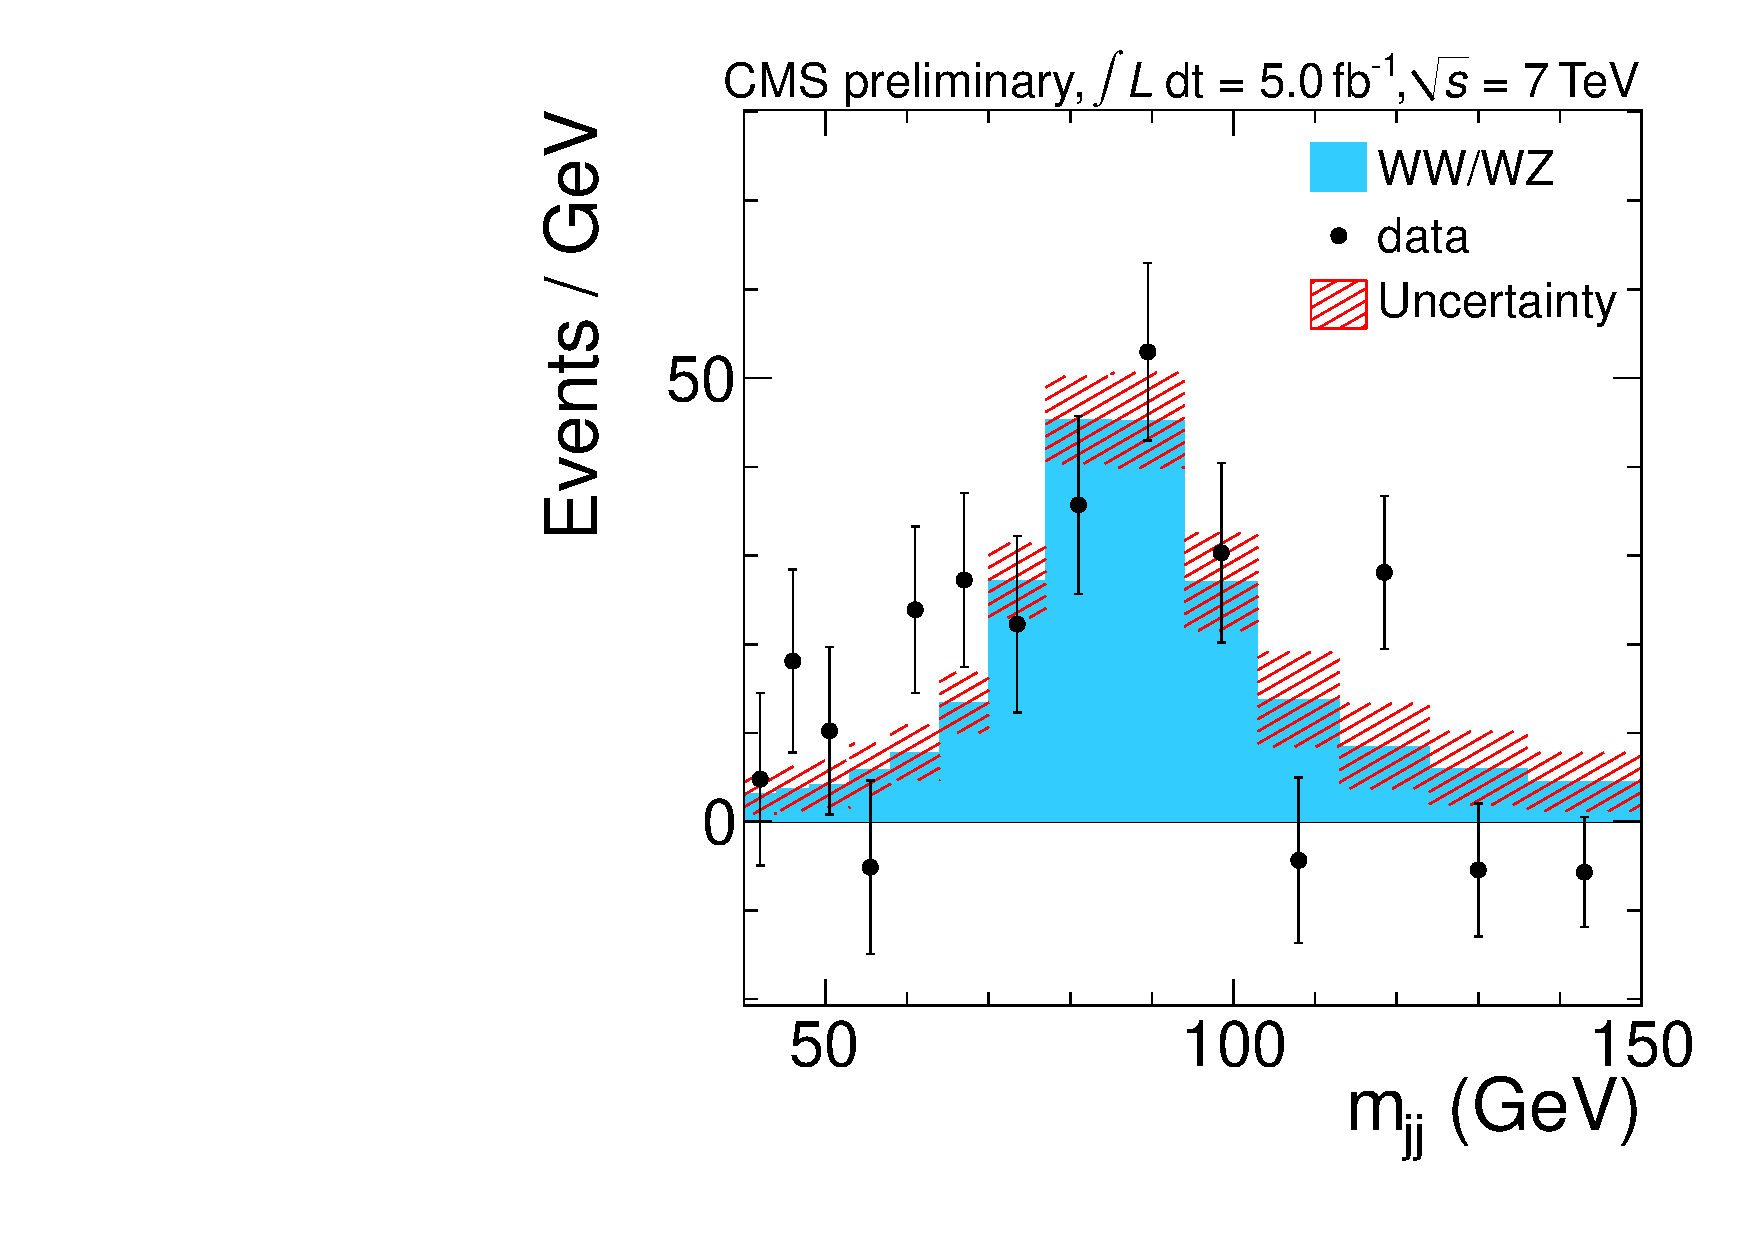
\includegraphics[width=0.49\textwidth]{figs/ScaleAndMatchingCrossChecks/mu2JNoBTag_fSUDeffMUm1sigma/Wjj_Diboson_Muon_2jets_Subtracted.pdf}
    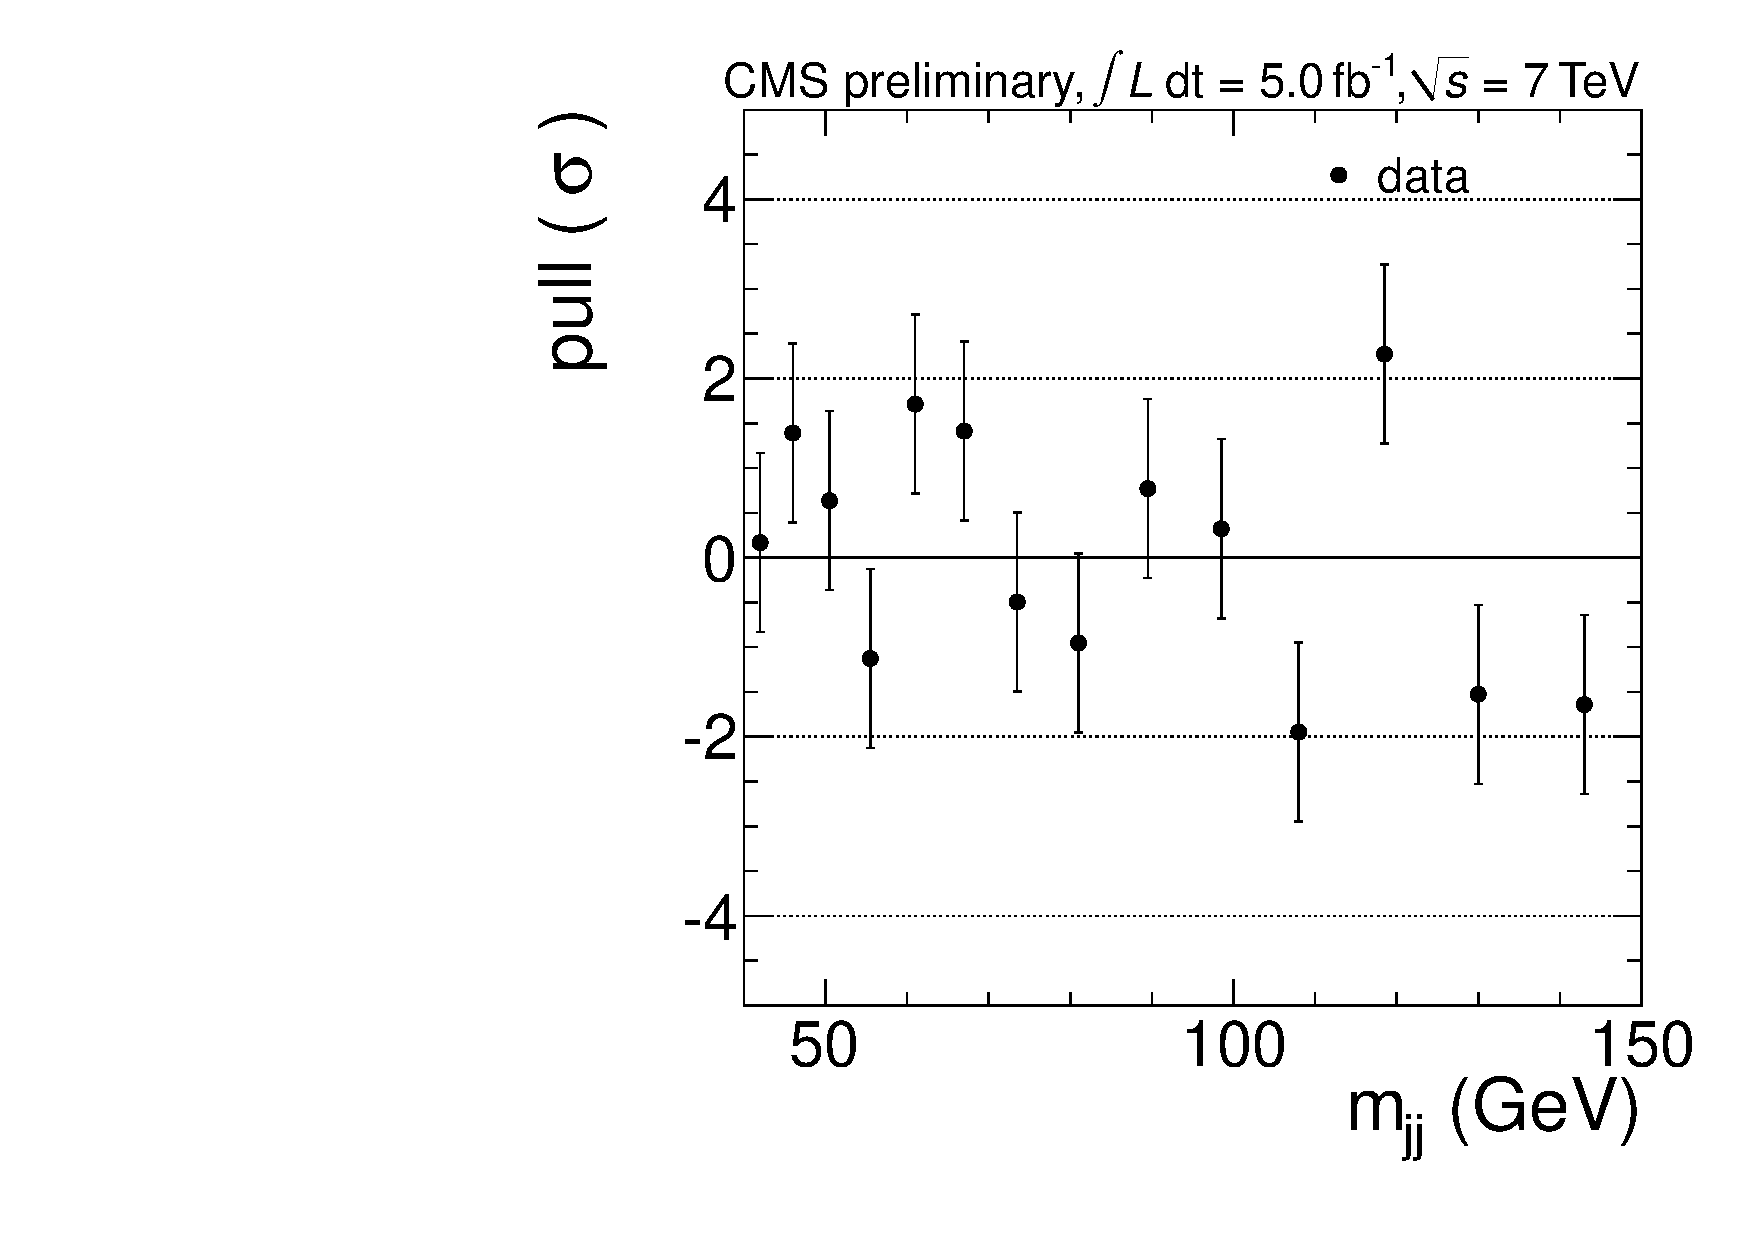
\includegraphics[width=0.49\textwidth]{figs/ScaleAndMatchingCrossChecks/mu2JNoBTag_fSUDeffMUm1sigma/Wjj_Diboson_Muon_2jets_Pull.pdf}
    \caption{Distribution of the dijet invariant mass for the non-b-tagged 2-jet events in muon data and Monte Carlo with $f_{MU}$ changed by $-1\sigma$: 
      (upper left) All background components stacked together, 
      (upper right) unstacked, (lower left) [Data minus all backgrounds except diboson],  
      (lower right) normalized residual between data and MC. }
    \label{fig:fsufmuXcheck_fSUDeffMUm1sigma}}
\end{figure}
%%%%%%%%%%%%%%%%%%%%
%%%%%%%%%%%%%%%%%%%%
\begin{figure}[h!]
  {\centering
    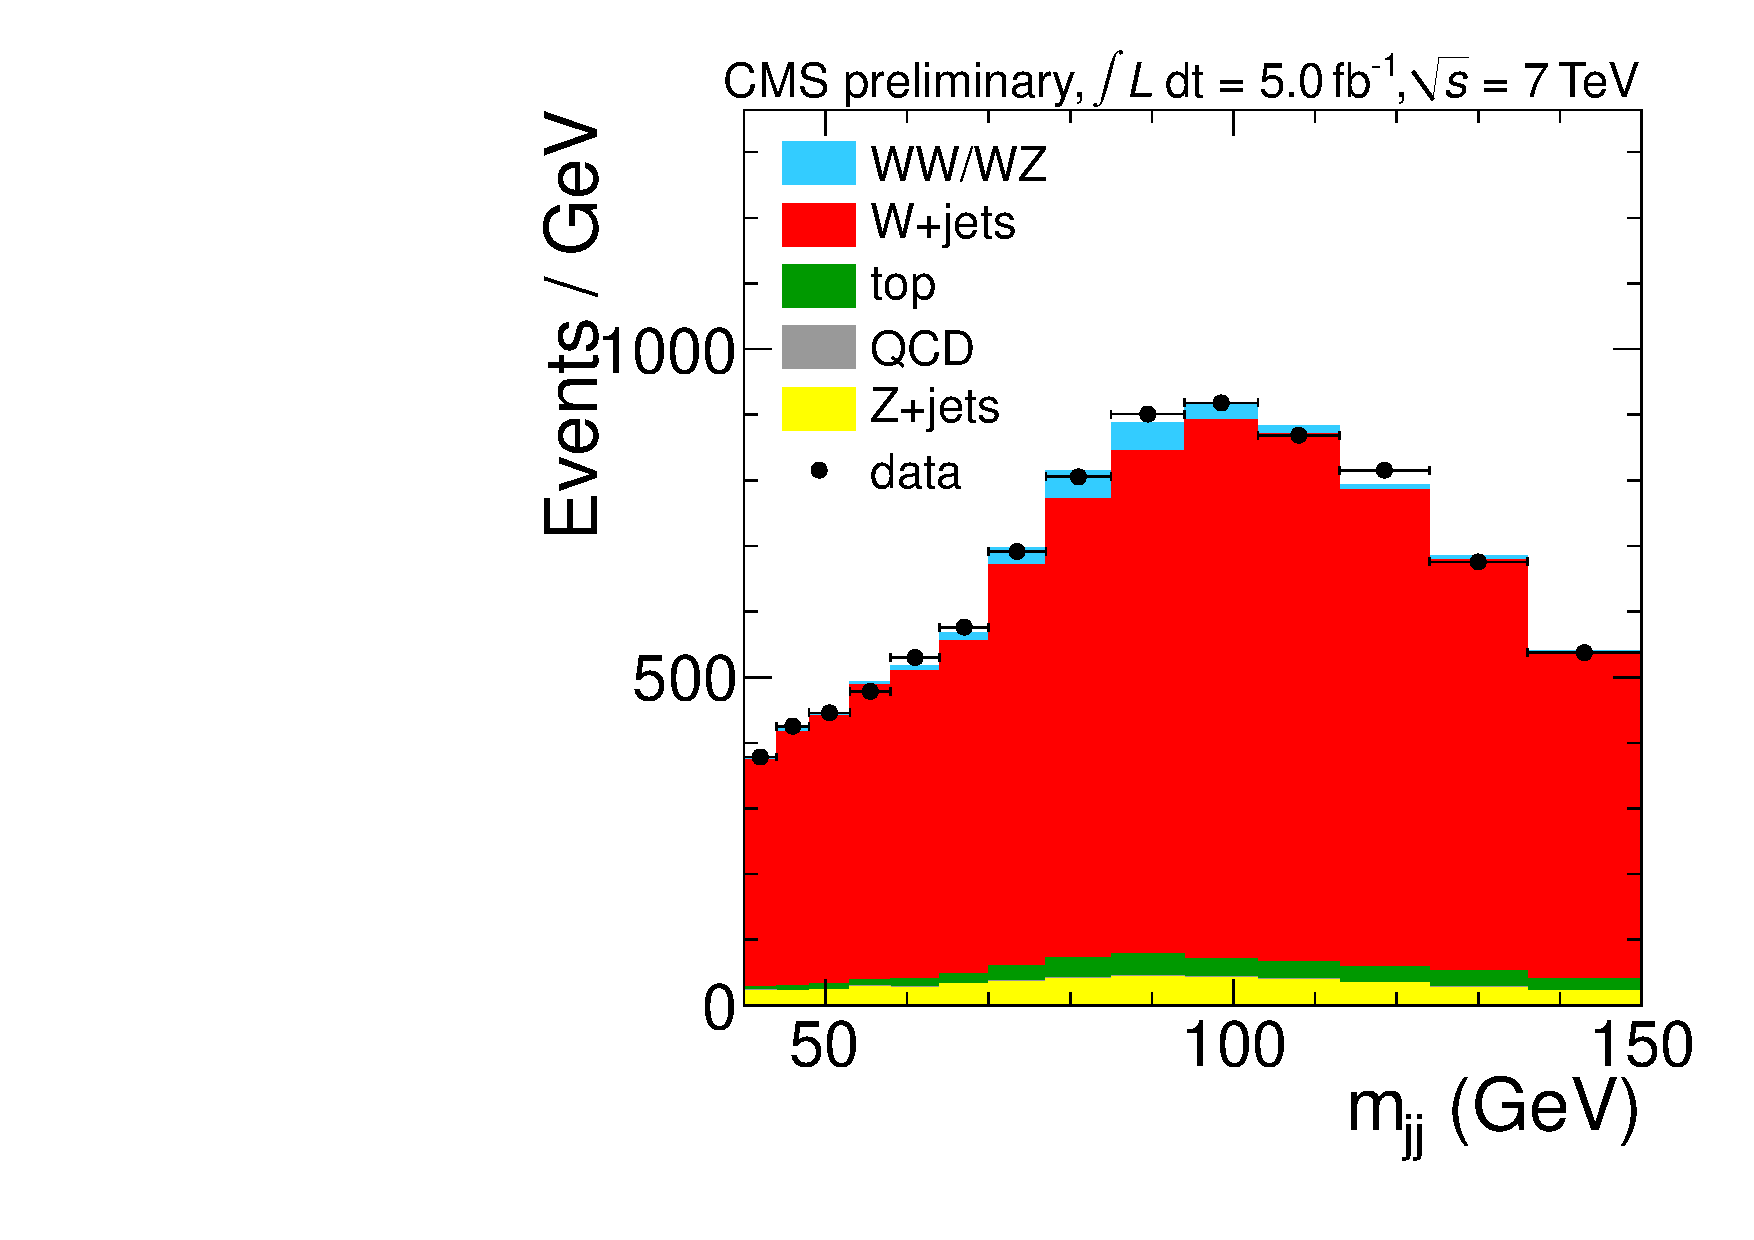
\includegraphics[width=0.49\textwidth]{figs/ScaleAndMatchingCrossChecks/mu2JNoBTag_fSUDeffMUp1sigma/Wjj_Diboson_Muon_2jets_Stacked.pdf}
    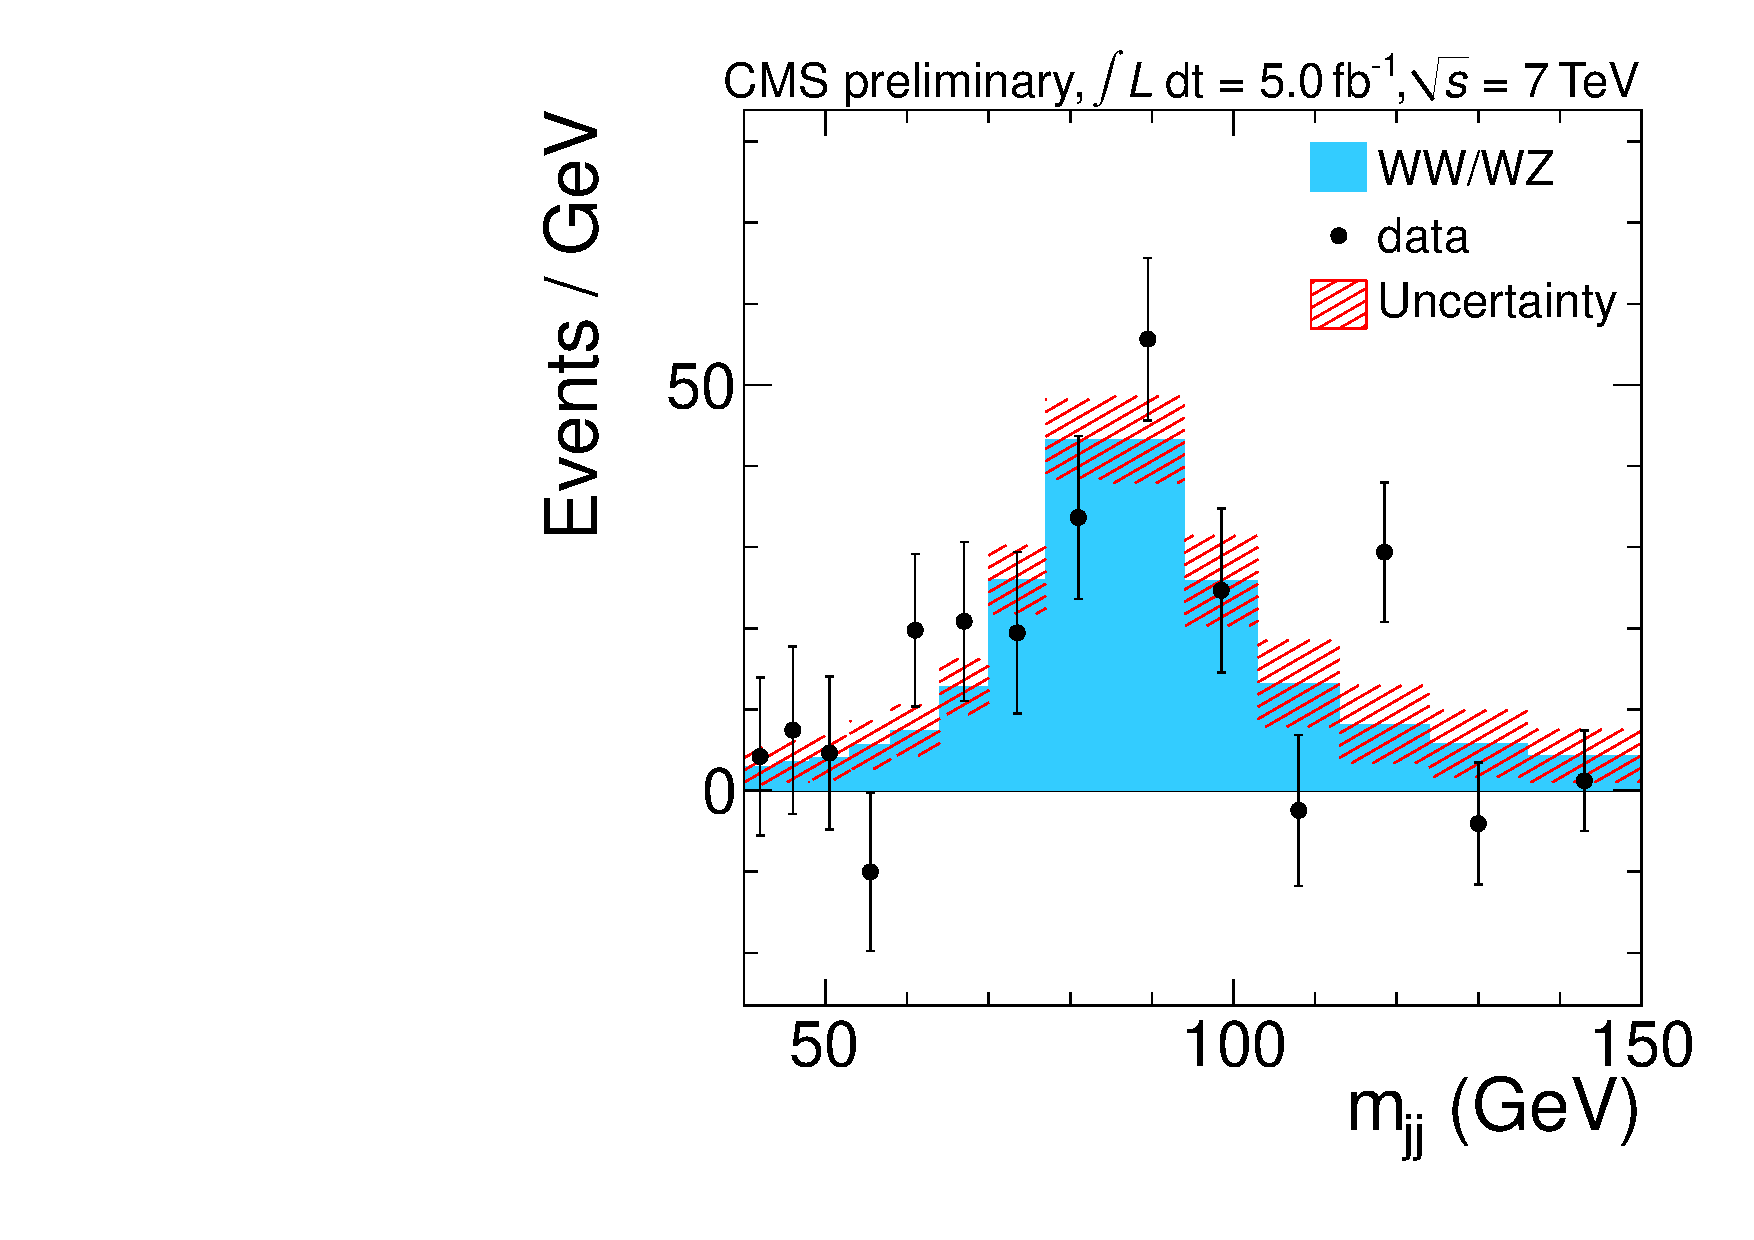
\includegraphics[width=0.49\textwidth]{figs/ScaleAndMatchingCrossChecks/mu2JNoBTag_fSUDeffMUp1sigma/Wjj_Diboson_Muon_2jets_Subtracted.pdf}
    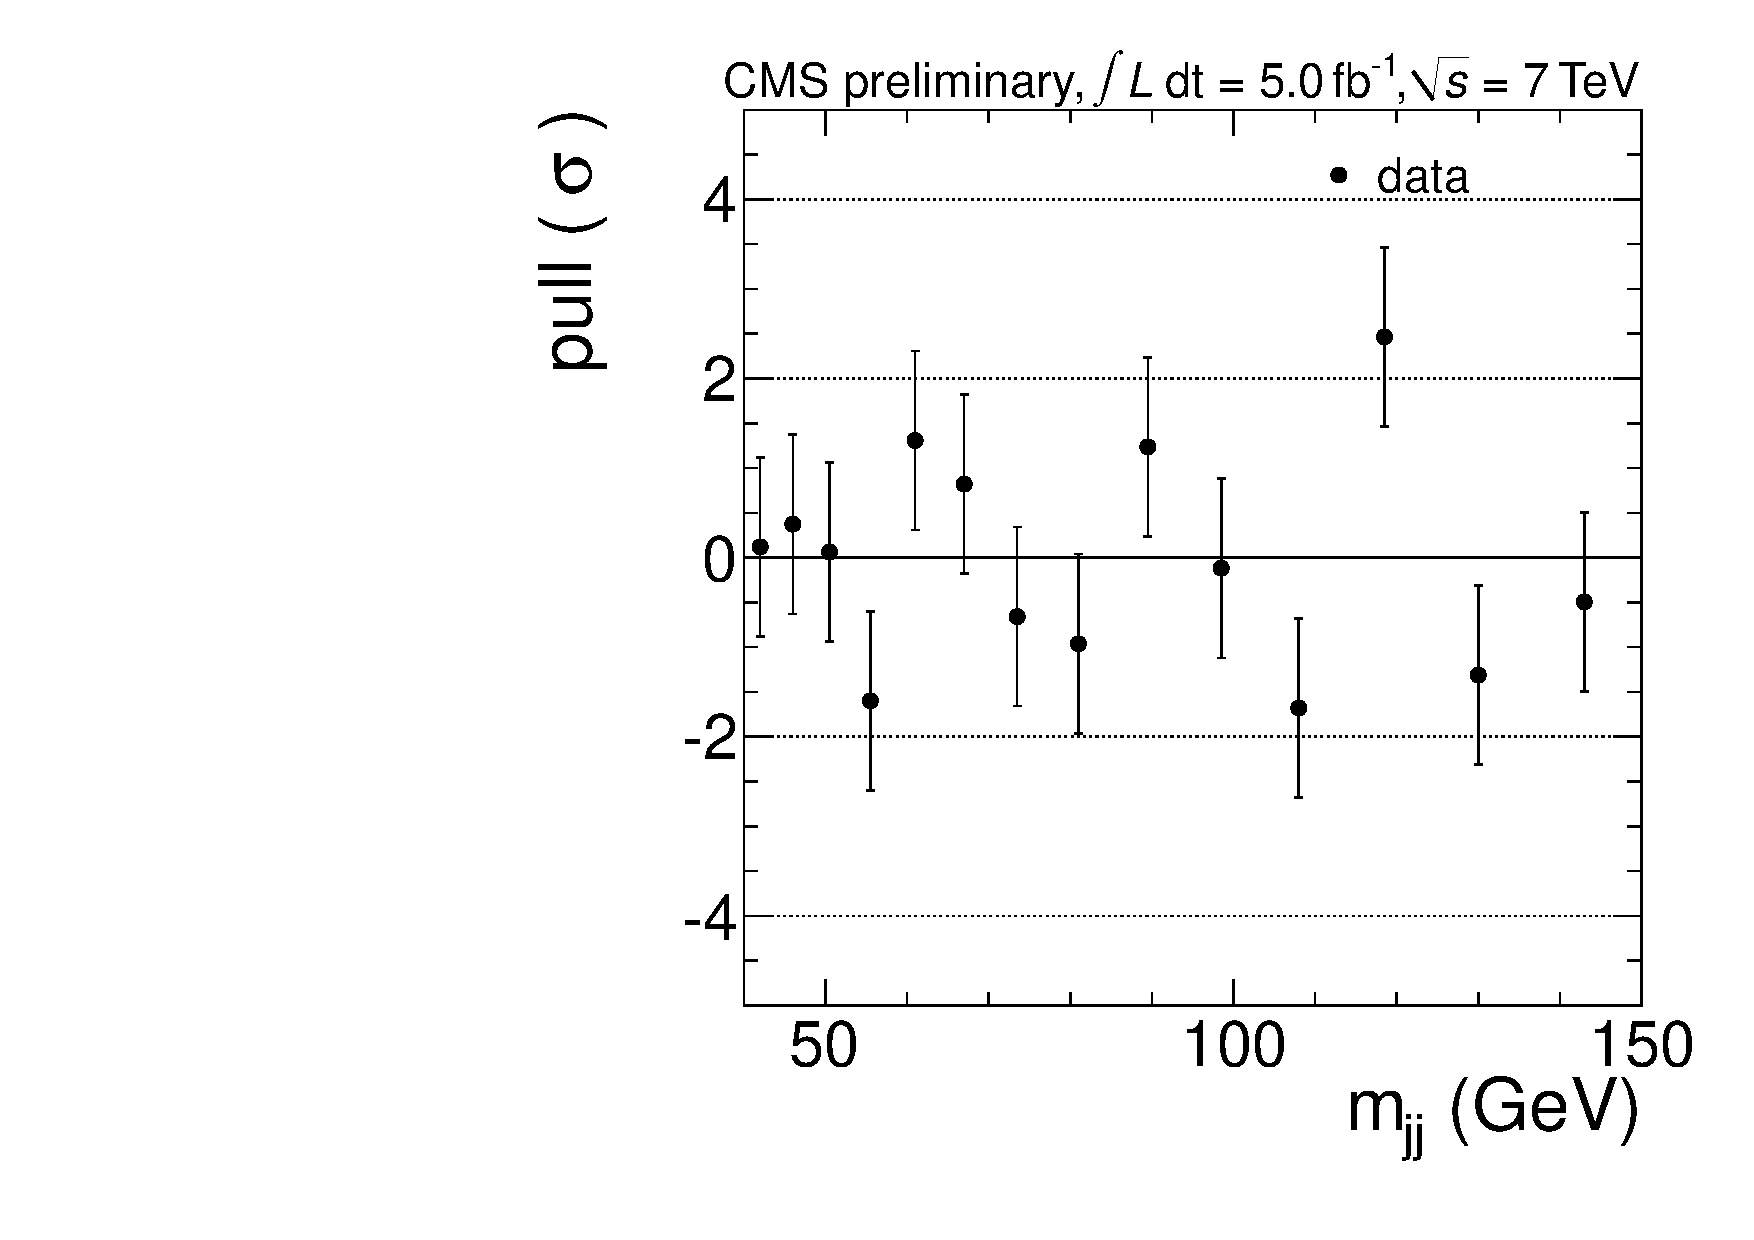
\includegraphics[width=0.49\textwidth]{figs/ScaleAndMatchingCrossChecks/mu2JNoBTag_fSUDeffMUp1sigma/Wjj_Diboson_Muon_2jets_Pull.pdf}
    \caption{Distribution of the dijet invariant mass for the non-b-tagged 2-jet events in muon data and Monte Carlo with $f_{MU}$ changed by $+1\sigma$: 
      (upper left) All background components stacked together, 
      (upper right) unstacked, (lower left) [Data minus all backgrounds except diboson],  
      (lower right) normalized residual between data and MC. }
    \label{fig:fsufmuXcheck_fSUDeffMUp1sigma}}
\end{figure}
%%%%%%%%%%%%%%%%%%%%
%%%%%%%%%%%%%%%%%%%%
\begin{figure}[h!]
  {\centering
    \includegraphics[width=0.49\textwidth]{figs/ScaleAndMatchingCrossChecks/el2JNoBTag_fMUfSUMuonDefault/Wjj_Diboson_Muon_2jets_Stacked.pdf}
    \includegraphics[width=0.49\textwidth]{figs/ScaleAndMatchingCrossChecks/el2JNoBTag_fMUfSUMuonDefault/Wjj_Diboson_Muon_2jets_Subtracted.pdf}
    \includegraphics[width=0.49\textwidth]{figs/ScaleAndMatchingCrossChecks/el2JNoBTag_fMUfSUMuonDefault/Wjj_Diboson_Muon_2jets_Pull.pdf}
    \caption{Distribution of the dijet invariant mass for the non-b-tagged 2-jet events in muon data and Monte Carlo with muon fit parameters applied to the electron sample: 
      (upper left) All background components stacked together, 
      (upper right) unstacked, (lower left) [Data minus all backgrounds except diboson],  
      (lower right) normalized residual between data and MC. }
    \label{fig:fsufmuXcheck_fMUfSUMuonDefault}}
\end{figure}
%%%%%%%%%%%%%%%%%%%%

\clearpage
